\documentclass[11pt]{article}
\usepackage[utf8]{inputenc}
\usepackage[T1]{fontenc}
\usepackage{amsmath,amssymb,amsthm,mathtools}
\usepackage{libertinus-otf}
\usepackage[margin=1in]{geometry}
\usepackage{graphicx,booktabs,array,longtable}
\usepackage{microtype}
\usepackage[numbers,sort&compress]{natbib}
\usepackage[hidelinks]{hyperref}
\usepackage{enumitem}
\setlist{itemsep=3pt,topsep=5pt}
\setlength{\emergencystretch}{2em}
\allowdisplaybreaks[2]
\numberwithin{equation}{section}
\newtheorem{theorem}{Theorem}[section]
\newtheorem{proposition}[theorem]{Proposition}
\newtheorem{corollary}[theorem]{Corollary}
\newtheorem{lemma}[theorem]{Lemma}
\theoremstyle{definition}
\newtheorem{definition}[theorem]{Definition}
\newtheorem{assumption}[theorem]{Assumption}
\newtheorem{example}[theorem]{Example}
\theoremstyle{remark}
\newtheorem{remark}[theorem]{Remark}
\newcommand{\E}{\mathbb E}
\newcommand{\R}{\mathbb R}
\newcommand{\Q}{\mathbb Q}
\newcommand{\F}{\mathcal F}
\newcommand{\G}{\mathcal G}
\newcommand{\ind}{\mathbf 1}
\newcommand{\dd}{\,\mathrm d}
\newcommand{\cE}{\mathcal E}
\DeclareMathOperator{\Var}{Var}
\DeclareMathOperator{\Cov}{Cov}
\DeclareMathOperator{\rank}{rank}
\DeclareMathOperator{\spanop}{span}
\DeclareMathOperator{\diag}{diag}
\DeclareMathOperator{\supp}{supp}
\newcommand{\norm}[1]{\left\lVert#1\right\rVert}
\newcommand{\abs}[1]{\left|#1\right|}
\newcommand{\lean}[1]{\texttt{\detokenize{#1}}}
\hypersetup{pdftitle={Forward curves with scheduled dates: consistency, realizations, and correlation}}
\title{Forward curves with scheduled dates:\\ consistency, realizations, and correlation}
\date{September 27, 2026}
\begin{document}
\maketitle
\begin{abstract}
Forward curves often distinguish maturities before and after scheduled policy meetings. We ask when a curve model with these breaks can retain its shape while satisfying the bond-pricing drift and announcement conditions. We show that announcement changes linear in maturity require Gaussian conditional laws after an explicit reweighting by earlier bond-price changes. For continuous one-factor dynamics with a fixed matrix-exponential maturity function, a state of fixed size can serve every meeting calendar exactly when the meeting loadings satisfy a finite linear recurrence. We construct that state and bound forward-rate and bond-price errors when recurrent loadings approximate a desired sequence. Finally, for the sum of a piecewise-linear meeting curve and a smooth exponential-polynomial curve, we characterize the permitted covariance and give the required meeting-curve drifts. A three-exponent construction has stochastic variance recoverable from the curve and true discounted-bond martingales. The splice specializes to explicit Svensson covariance restrictions; for uncorrelated blocks with positive moving decays, the classical exponent restrictions remain unchanged.
\end{abstract}
\noindent\textbf{Keywords:} term structure; scheduled dates; HJM consistency; finite-dimensional realization; exponential-polynomial family.

\section{Introduction}
Central banks change policy rates at scheduled meetings. An interest-rate model should therefore distinguish a loan that ends before a meeting from one that extends beyond it. A forward curve can express this distinction by having a different level on either side of the meeting date. As news arrives, those levels change. At the meeting itself, the announcement may cause another change.

The difficulty is to make these movements compatible with bond prices. Consider the simplest proposed model: the forward curve is constant between consecutive meetings, and each of its levels fluctuates randomly. This is easy to describe and to fit. Yet the usual no-arbitrage drift restriction does not preserve it. Even if volatility is constant across maturities within an interval, the required drift increases linearly across that interval. The curve acquires a slope. A model that insists on keeping every interval flat must eliminate that volatility.

This example illustrates the question studied here: \emph{which models of a forward curve with scheduled dates can retain their chosen shape as they evolve?} Retaining the shape is useful because it allows the entire curve to be represented by a small number of parameters. Compatibility with the drift restriction is necessary because the same evolving curve determines the prices of bonds of every maturity. We call a family \emph{consistent} when its dynamics satisfy the drift and announcement restrictions while remaining within the family.

There are two distinct ways in which a meeting enters this question. First, the curve observed today may have a break at the meeting's maturity date: rates applying before and after the meeting differ. Second, when the meeting occurs, new information may change rates for a fixed future maturity. A break in today's curve does not by itself describe an unexpected announcement. We treat these two mechanisms separately.

\subsection{Questions and results}
\paragraph{What shape can an announcement produce?}
Suppose an announcement changes the forward curve by a random level together with a maturity-dependent correction known immediately before the announcement. The correction is needed because bond prices depend exponentially on the integral of forward rates: a mean-zero rate change need not produce a mean-zero bond-price change. We show that the distribution of the random level determines the correction. If the correction is a straight line in maturity, that distribution must be Gaussian. Across several meeting intervals, the same conclusion applies after reweighting outcomes by the bond-price change accumulated over the preceding intervals. We state this reweighting explicitly in Section~\ref{sec:jumps}. It permits announcement vectors that are not jointly Gaussian. A nondegenerate hike/no-hike outcome, in contrast, is exactly incompatible with the prescribed piecewise-linear jump shape. That is a classification result rather than a large pricing effect: for the symmetric 25-basis-point example, the exact correction and its Gaussian tangent differ by only about $8\times10^{-9}$ basis points at one year. A discrete policy outcome can therefore be economically natural and numerically almost indistinguishable from the convenient affine approximation.

\paragraph{When can a fixed number of state variables describe the curve?}
Now consider continuous changes in forward rates between announcements. A common specification assigns a volatility loading according to how many meetings lie between today and the maturity. Thus one sequence of numbers specifies the sensitivity before the next meeting, between the next two meetings, and so on. A smooth maturity function, such as exponential decay, multiplies those loadings.

For any fixed finite calendar, one can keep adding state variables until the model records all past shocks that affect future maturities. A different question is whether the same state architecture remains available as the calendar grows. For one Brownian factor, constant volatility scale, and a nonzero maturity function with a finite matrix-exponential representation, we prove that it does precisely when the loading sequence satisfies a finite linear recurrence. A recurrence allows subsequent loadings to be obtained from a fixed number of preceding ones. It also allows past shocks to be summarized by a fixed number of state variables.

For example, loadings $1-\theta^i$, where $i$ is the number of intervening meetings and $0<\theta<1$, satisfy a second-order recurrence. They admit a state representation whose size does not grow with the calendar. The cumulative loadings $1+1/2+\cdots+1/i$ satisfy no finite recurrence and admit no such exact representation. Section~\ref{sec:realizations} proves both the obstruction and the construction. A complementary two-factor example in Section~\ref{sec:varianceexample} keeps only three exponential coefficients while making stochastic variance recoverable from the curve itself. Its discounted bonds are true martingales; the example shows that a stochastic coefficient on a drift-generated maturity shape need not force an unlimited enlargement of the family.

\paragraph{Can a small model still approximate a sequence with no recurrence?}
Exact representation across every calendar is a strong requirement. For a specified finite calendar, a short sum of geometric sequences may approximate the desired loadings accurately. Each such sum satisfies a recurrence. We show how its maximum loading error controls mean-square errors in forward rates and bond prices. Each model uses the drift required by its own volatility. The constants depend on the horizon and the sizes of the loadings and maturity function, without a separate dependence on the number or spacing of meetings. Section~\ref{sec:examples} applies the result to the cumulative loadings above and compares the bounds with computed errors.

\paragraph{How can meeting effects be combined with a smooth curve model?}
A model may add a curve that is linear between meetings to a smooth component, such as a sum of polynomial and exponential functions of time to maturity. The two components may share shocks. Their covariance then contributes to the required drift, so two separately admissible specifications need not remain admissible when combined.

We characterize the allowed covariance. At each maturity breakpoint, the change in the total meeting-related volatility must have zero instantaneous covariance with every nonconstant coordinate of the smooth component. A constant level is the exception. There is also a restriction within the smooth component: its covariance must be evaluated using the combined level noise of both components. With these restrictions, we give the drifts of the piecewise-linear component that satisfy the full drift equation. Section~\ref{sec:splice} develops this criterion, starting from the separate drift contributions and showing where the covariance enters. The Svensson specialization identifies the extra level covariance that the meeting component permits. For an uncorrelated block with strictly positive but potentially moving decay parameters, we also prove that its full standalone consistency equation survives: adding the meeting component does not relax the classical restrictions on those decays.

\subsection{Relation to the literature}
\paragraph{Policy meetings and overnight rates.}
The economic role of policy meetings in the term structure predates the transition to SOFR. \citet{piazzesi2005bond} models the policy target as a jump process with meeting-day effects on jump intensity. Those jumps occur at random times with elevated intensity on meeting days; this differs from an atom at an exact announcement time. \citet{das2002surprise} also allows meeting days to affect jump probabilities. Models with genuinely scheduled random-size announcements include \citet{kim2014jumps,backwell2021expected}; discrete scheduled outcomes are treated by \citet{silva2024discretely}. These models specify rate dynamics and derive prices. Our question instead fixes a maturity family and asks which dynamics preserve it.

For overnight-rate curves, \citet{gellert2021short} uses step volatilities at meeting maturities and combines the meeting component with an independent smooth component. \citet{brace2024sofr} adds stochastic volatility, exponential decay, and calibration to futures and options. Its continuous fixed-maturity forward dynamics can produce scheduled short-rate jumps by crossing maturity breakpoints. That mechanism is distinct from the additional announcement variables $\xi_n$ studied here. Our covariance criterion extends the independent combination by identifying the correlations compatible with its prescribed maturity shapes. Our finite-calendar example in Section~\ref{sec:combined} includes both diffusion and nonzero announcement changes.

\paragraph{Drift restrictions and announcement transforms.}
The continuous drift restriction is the HJM condition of \citet{heath1992bond}. \citet{fontana2018term} extends term-structure modeling to fixed discontinuity dates in a multiple-curve setting. \citet[Theorem 3.5, Remark 3.9]{fontana2022term} gives the overnight-rate formulation specialized in Section~\ref{sec:setting}. \citet{kellerressel2018affine} gives related conditions for affine semimartingales with a deterministic clock that may have atoms.

Exponential transforms and Gaussian scheduled jumps are established ingredients: see \citet{kellerressel2018affine}, \citet[Example 3.10 and Section 4.3]{fontana2022term}, and \citet[Proposition 1]{kim2014jumps}. The log-Laplace identity in Proposition~\ref{prop:profile} is a direct consequence of the jump condition. The particular conclusion developed here is the converse for a piecewise-affine jump family: each interval level must be centered Gaussian under the preceding intervals' bond-price tilt. The non-jointly-Gaussian example shows why this conclusion is weaker than requiring one jointly Gaussian announcement vector. The quantitative two-point example explains why this exact restriction can have a negligible effect at realistic rate scales.

\paragraph{Consistency of smooth curve families.}
\citet{bjork1999interest} characterizes invariance of parametric curve families, and \citet{filipovic1999note} establishes the Nelson--Siegel obstruction. \citet{filipovic2000exponential,sharef2004conditions} study exponential-polynomial families; \citet{filipovic2001consistency} develops the general consistency framework. The geometric approach to finite-dimensional invariant manifolds is developed by \citet{filipovic2004geometry}, including external stochastic factors, and extended to Wiener--Poisson jump-diffusions by \citet{filipovic2012invariant}. Scheduled maturity breakpoints require the drift identity to hold for the different analytic expressions on adjacent intervals.

The meeting component can absorb a discrepancy that is affine in maturity, so the smooth-block residual need only be affine rather than zero. With correlation it must be computed at the combined level covariance. Section~\ref{app:blocks} makes the consequence concrete: a Nelson--Siegel block can carry a stochastic level when its linear drift residual is absorbed by the front end, while its exponential shape coordinates remain restricted. The Svensson corollary likewise retains the classical exponent resonance while allowing a level correlated with its exponential-level coordinate. Theorem~\ref{thm:varyingexponents} treats a different extension, in which the decay parameters are coordinates of the state. It transfers the restrictions of \citet{filipovic2000exponential} to an uncorrelated scheduled splice with positive decays. The transfer and the explicit added covariance are the contributions; the block-alone restrictions are established results.

\paragraph{Hankel rank and realization theory.}
The linear-algebra ingredients are classical. \citet[Propositions 1--2 and Theorem 1]{hokalman1966effective} characterizes matrix sequences that admit a finite linear recurrence, identifies minimal realization dimension with Hankel rank, and constructs a realization from the sequence. Our representation of meeting loadings by powers of a matrix uses this theory.

The closest interest-rate precedent is \citet{bjork1999minimal}. For deterministic volatility that is a smooth function of time to maturity alone, its Proposition~3.1 characterizes finite-dimensional linear realizations by a matrix-exponential representation of the volatility. Proposition~4.1 identifies the minimal dimension with the span of its derivatives; Proposition~5.1 interprets the state through benchmark forward rates. The initial curve and deterministic HJM drift are supplied separately as a time-dependent output correction. Its point-process extension assumes a compensator proportional to calendar time (Assumption~7.1), so it does not include probability atoms at scheduled announcement dates.

Our volatility also depends on the number of intervening meetings. Its maturity breakpoints move as time passes, so it is outside that smooth, time-independent specification. We ask for one state dimension, one locally Lipschitz curve map, and one meeting-update rule serving every finite calendar and horizon. The additional result is that this requirement forces a recurrence of the meeting loadings, even when the curve map may be nonlinear. The sufficient construction combines continuous maturity translation with discrete meeting updates and records the HJM drift in the state. This is an extension of classical realization methods to the stated calendar convention; the recurrence algebra and the matrix-exponential maturity representation are established ingredients. Our displayed state is an upper bound, not a minimal-dimension formula. Section~\ref{sec:realizations} explains why its deterministic calendar memory must be distinguished from its random coordinates.

For smooth maturity dependence without meetings, \citet[Proposition 5.1 and Corollary 5.1]{bjork2001existence} and \citet[Corollary 8.1]{tappe2010alternative} identify the role of quasi-exponential functions. \citet{bjork2004finite} treats external stochastic-volatility states. Our sufficient construction combines those continuous-time translations with the discrete shifts of a recurrent meeting sequence. The approximation estimates use Gaussian stability and regenerate the HJM drift after replacing the loadings. They complement \citet{benth2018approximation}, whose finite-dimensional commodity-forward approximations use a Riesz basis and include convergence rates under additional regularity.

Section~\ref{sec:setting} defines the model and consistency conditions. Sections~\ref{sec:jumps}--\ref{sec:splice} develop the announcement, realization, approximation, and covariance results. Section~\ref{sec:examples} illustrates their numerical meaning. Supporting arguments are in the appendix.

\section{The forward-rate model}\label{sec:setting}
\subsection{Dates, rates, and bond prices}
We use $t$ for the date on which a curve is observed and $T$ for the maturity of a contract, with $0\le t\le T$. The instantaneous forward rate $f(t,T)$ is the rate observed at $t$ for an infinitesimal lending period starting at $T$. Its diagonal value $r_t=f(t,t)$ is the short rate. A zero-coupon bond paying one unit at $T$ has price
\begin{equation}
P(t,T)=\exp\left(-\int_t^T f(t,u)\dd u\right).
\label{eq:bonddefinition}
\end{equation}
Thus a change in the integral of the forward curve changes the logarithm of the bond price with the opposite sign. This relation is why the shape of the curve, rather than just its value at a few maturities, matters for consistency.

For statements on a particular calendar, fix a horizon $H>0$. Section~\ref{sec:realizations} explicitly quantifies over all finite horizons when asking for one realization serving every schedule. There are $N$ scheduled meetings, at deterministic dates $T_1,\ldots,T_N$. Set
\[
0=T_0<T_1<\cdots<T_N<H=T_{N+1},\qquad I_k=[T_k,T_{k+1}).
\]
The interval $I_k$ is the range of maturities between meetings $k$ and $k+1$; $T_0$ and $T_{N+1}$ are boundary dates, not additional meetings. At a given time $t<H$, let $j(t)$ be the unique index with $t\in I_{j(t)}$. We take values at interval endpoints from the right.

\subsection{Continuous changes and announcements}
Work on a filtered probability space with pricing measure $Q$. The information available at $t$ is $\F_t$; the information just before meeting $T_n$ is $\F_{T_n-}$. The filtration satisfies the usual conditions. Let $W$ be a vector of independent Brownian motions, representing continuously arriving shocks.

For each fixed maturity $T$, the initial rate is $f_0(T)$. Between meetings its drift is $\alpha(t,T)$ and its vector of Brownian sensitivities is $\sigma(t,T)$. At meeting $T_n$, define the announcement change
\[
\xi_n(T)=f(T_n,T)-f(T_n-,T),\qquad T\ge T_n.
\]
This is a random function of the remaining maturity $T$. With this notation the evolution is
\begin{equation}
f(t,T)=f_0(T)+\int_0^t\alpha(s,T)\dd s
 +\int_0^t\sigma(s,T)\cdot\dd W_s
 +\sum_{T_n\le t}\xi_n(T).
\label{eq:hjm}
\end{equation}
The four terms are the initial curve, accumulated drift, accumulated continuous shocks, and accumulated announcement changes. The dot denotes the Euclidean inner product. Coefficients have the measurability and local integrability required for these integrals; more specific conditions are stated with each result. We use the standard stochastic integral and It\^o formula; see \citet{revuz1999continuous}.

Figure~\ref{fig:discontinuities} distinguishes the two kinds of discontinuity. Holding $t$ fixed, the function $T\mapsto f(t,T)$ may have a break at a future meeting date $T_n$. It assigns different rates to periods before and after that meeting. Holding $T$ fixed instead, the function $t\mapsto f(t,T)$ may jump when the announcement arrives; that jump is $\xi_n(T)$.

For example, a curve can be flat at one rate before the next meeting and at another rate afterward, while both levels evolve continuously before the meeting. This curve has a maturity breakpoint. If every fixed-maturity rate also remains continuous through the meeting, then $\xi_n=0$, although the short rate can jump as it passes from the first interval to the second. That short-rate jump is known immediately before the date in the continuous-filtration models used below. Section~\ref{sec:jumps} studies nonzero announcement changes. Sections~\ref{sec:realizations}--\ref{sec:splice} set them to zero and study the dynamics of maturity breakpoints.

\begin{figure}[htbp]
\centering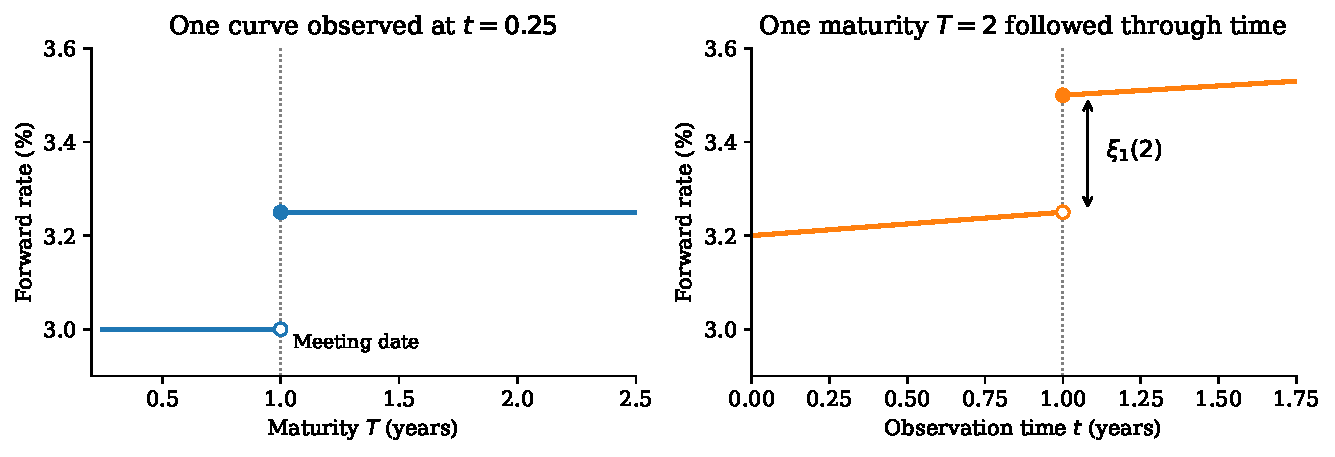
\includegraphics[width=\linewidth]{figures/two_discontinuities.pdf}
\caption{Two different meanings of a meeting-date discontinuity. Left: at one observation time, the forward curve assigns different rates to maturities before and after a future meeting. Right: for one fixed maturity, the rate changes when an announcement arrives. These are schematic illustrations of the two axes, not paths generated by a calibrated model.}\label{fig:discontinuities}
\end{figure}

\subsection{The restrictions imposed by bond prices}
The bank account is $B_t=\exp(\int_0^t r_s\dd s)$. Under the pricing measure, discounted bond prices $P(t,T)/B_t$ must have zero local drift. Between announcements, It\^o's formula applied to \eqref{eq:bonddefinition} gives the following restriction, the integrated form of the drift condition of \citet{heath1992bond}.

\begin{assumption}[Integrated drift condition]\label{ass:drift}
For every maturity $T$, for $Q\otimes dt$-almost every $(\omega,t)$ with $t\le T$,
\begin{equation}
\int_t^T\alpha(t,u)\dd u
 =\frac12\left|\int_t^T\sigma(t,u)\dd u\right|^2.
\label{eq:drift}
\end{equation}
\end{assumption}
The integral on the right is the bond's Brownian sensitivity, up to sign. Its squared norm supplies the It\^o correction. Thus volatility determines the integrated forward drift. Wherever maturity differentiation is valid, the equivalent pointwise formula is
\begin{equation}
\alpha(t,T)=\sigma(t,T)\cdot\int_t^T\sigma(t,u)\dd u.
\label{eq:diffdrift}
\end{equation}
This formula explains the elementary obstruction from the introduction. If $\sigma(t,T)=s$ is constant in maturity on an interval beginning at $t$, then $\alpha(t,T)=|s|^2(T-t)$ there. A constant volatility generates a sloping drift.

At an announcement, \eqref{eq:bonddefinition} gives the bond-price ratio
\[
\frac{P(T_n,T)}{P(T_n-,T)}
 =\exp\left(-\int_{T_n}^T\xi_n(u)\dd u\right).
\]
The bank account is continuous at $T_n$. The conditional expected bond-price ratio must therefore be one:
\begin{assumption}[Scheduled-jump condition]\label{ass:jump}
For every meeting $T_n$ and maturity $T\ge T_n$,
\begin{equation}
\E\left[\exp\left(-\int_{T_n}^T\xi_n(u)\dd u\right)
 \middle|\F_{T_n-}\right]=1\quad Q\text{-a.s.}
\label{eq:jump}
\end{equation}
\end{assumption}
Here $\E$ means expectation under $Q$. This is a restriction on the distribution of the entire integrated announcement change. Requiring only that the rate change have conditional mean zero would not suffice, because the exponential is nonlinear.

These two conditions specialize \citet[Theorem 3.5 and Remark 3.9]{fontana2022term} to the bond definition \eqref{eq:bonddefinition}, a continuous bank account, and finitely many deterministic announcement dates. In this paper, consistency means satisfaction of these conditions while remaining in the stated curve family. A true-martingale conclusion for discounted bonds additionally requires the corresponding integrability; local drift identities alone do not supply it.

\subsection{Curves that are linear between meetings}
The simplest extension of a curve that is flat between meetings allows a slope on each interval. For $T\in I_m$ write
\begin{equation}
f(t,T)=L_m(t)+C_m(t)(T-T_m),\qquad T\ge t.
\label{eq:front}
\end{equation}
The coefficient $L_m(t)$ is the level at the interval's left endpoint, and $C_m(t)$ is its slope as a function of maturity. A later interval has its own level and slope, so a break at a meeting is allowed. We denote this family by $S^+$ and its zero-slope subfamily by $S$.

In the diffusion models below, the levels have Brownian noise and the slopes have finite variation. Consequently volatility is constant in maturity on each interval, while drift can be linear there, as required by \eqref{eq:diffdrift}. Section~\ref{sec:splice} adds a smooth component to this piecewise-linear curve. We call the piecewise-linear component the \emph{front end} and the smooth component the \emph{block}; the sum is the \emph{splice}.

Equality of stochastic curve representations means almost-sure equality at each fixed $t,T$. For bond prices we use a jointly measurable maturity version, constructed in Section~\ref{sec:approximation}. The following elementary observation specifies the exceptional-set convention used in the drift proofs.

\begin{lemma}[A common exceptional set for maturities]\label{lem:maturitynull}
Suppose the drift and volatility are locally integrable in maturity and satisfy \eqref{eq:drift} for every fixed $T$, almost everywhere in time and probability. Then there is one time--probability exceptional set outside which the integrated identity holds for every $T\ge t$. If the drift and volatility are continuous inside each maturity interval, then for $T>t$, \eqref{eq:diffdrift} holds at every interior maturity outside that set.
\end{lemma}
\begin{proof}
Take the union of the exceptional sets for rational $T$, together with the set on which the maturity integrals fail to be defined. This is a null set. The primitives on both sides of \eqref{eq:drift} are continuous in $T$, so agreement on rational maturities extends to all maturities. On an interval with continuous coefficients, differentiation gives \eqref{eq:diffdrift} throughout its interior.
\end{proof}

\section{The shape of a scheduled jump}\label{sec:jumps}
What adjustment to the forward curve is needed when a meeting reveals a random rate change? The answer follows from the bond-price ratio in \eqref{eq:jump}. We first consider a single random level affecting all remaining maturities, and then allow a different level on each meeting interval.

\subsection{The correction required by a random level change}
Fix meeting $T_n$ and write $\G=\F_{T_n-}$ for the information available immediately before it. Let $u\ge0$ denote time from the meeting to maturity. The announcement reveals a scalar random variable $X$. Suppose it changes every remaining forward rate by $X$, plus a function $h(u)$ already known given $\G$. Thus $h$ is the maturity-dependent correction accompanying the level change. For a bond maturing $\tau$ units of time after the meeting, denote the integrated correction by $\mathcal H(\tau)$:
\[
\xi_n(T_n+u)=X+h(u),\qquad \mathcal H(\tau)=\int_0^\tau h(u)\dd u.
\]
We assume $h$ is locally integrable. The bond-price ratio is $\exp(-\tau X-\mathcal H(\tau))$. Setting its conditional expectation to one gives
\[
 e^{-\mathcal H(\tau)}\E[e^{-\tau X}\mid\G]=1.
\]
Consequently the integral of the correction must equal the logarithm of the conditional exponential moment of $X$. Denote that logarithm by
\[
\mathcal L_X(\tau)=\log\E[e^{-\tau X}\mid\G].
\]
The function $\mathcal L_X$ is the conditional log-Laplace transform. We assume a regular conditional law of $X$ given $\G$ and take the domain $0\le\tau\le H-T_n$. The scheduled-jump condition forces this transform to be finite throughout that domain, since $\mathcal H$ is finite there. For the converse, assume this finiteness. For $\tau$ in the interior, define the expectation under its exponential tilt by
\[
\E_\tau[g(X)\mid\G]
 =\frac{\E[g(X)e^{-\tau X}\mid\G]}{\E[e^{-\tau X}\mid\G]}.
\]
The tilt gives greater weight to outcomes with a smaller level change, which produce a larger bond-price ratio. Let $\Var_\tau$ denote variance under the same conditional law.

\begin{proposition}\label{prop:profile}
The scheduled-jump condition is equivalent to $\mathcal H(\tau)=\mathcal L_X(\tau)$ for every $\tau\in[0,H-T_n]$. On the interior, the correction has the smooth representative
\begin{equation}
h(\tau)=\mathcal L_X'(\tau)=-\E_\tau[X\mid\G],\qquad
h'(\tau)=\mathcal L_X''(\tau)=\Var_\tau(X\mid\G)\ge0.\label{eq:profile}
\end{equation}
In particular, for coefficients $h_0,y$ known given $\G$, a straight-line correction $h(u)=h_0+yu$ satisfies the jump condition precisely when the conditional distribution of $X$ is Gaussian with mean $-h_0$ and variance $y\ge0$.
\end{proposition}
The first derivative determines the correction; the second says that its slope is a variance and therefore nonnegative. For example, if $X$ is conditionally Gaussian with mean zero and variance $v$, the required correction is $h(u)=vu$. Its integrated value $v\tau^2/2$ exactly cancels the Gaussian exponential moment $\E[e^{-\tau X}\mid\G]=e^{v\tau^2/2}$. Thus uncertainty about a level change produces an upward slope in the announcement profile.

\begin{proof}
The conditional expectation in \eqref{eq:jump} is $e^{-\mathcal H(\tau)}\E[e^{-\tau X}\mid\G]$. Its equality to one gives the first statement. Finiteness on an open interval permits differentiation on compact subintervals, yielding the conditional mean and variance formulas. If $\mathcal H=h_0\tau+y\tau^2/2$, the conditional transform is the Gaussian transform. Uniqueness of a Laplace transform on an interval gives the stated law, including the degenerate case $y=0$. Conversely that law gives the required transform. Equalities initially imposed at rational maturities extend by continuity; $h=\mathcal L_X'$ is understood almost everywhere when only local integrability was assumed.
\end{proof}

Other distributions give different correction shapes. The next example makes that correspondence explicit.

\begin{example}[A two-point announcement]\label{ex:binary}
Let $X=\Delta$ with conditional probability $\pi$ and $X=0$ otherwise, with $0<\pi<1$. Its admissible profile is
\begin{equation}
h(\tau)=-\Delta\frac{\pi e^{-\tau\Delta}}{1-\pi+\pi e^{-\tau\Delta}}.
\end{equation}
The affine profile with the same value and derivative at zero is $-\pi\Delta+\pi(1-\pi)\Delta^2\tau$. For $\pi=1/2$ and $\Delta>0$, the affine profile exceeds the exact one by
\[
g(\tau)=\frac\Delta2\left(\frac{\Delta\tau}{2}-\tanh\frac{\Delta\tau}{2}\right),
\qquad 0\le g(\tau)\le\frac{\Delta^4\tau^3}{48}.
\]
The bound follows by integrating $1-\operatorname{sech}^2 z=\tanh^2z\le z^2$. Thus a shape restriction can distinguish the distributions exactly while their admissible curves are extremely close at small rate scales. Figure~\ref{fig:jumps} quantifies this distinction.
\end{example}

\subsection{Several maturity intervals}
A meeting may change near and distant forward rates by different amounts. Keep the announcement date $T_n$ fixed, and let $X_k$ be its random level change on maturity interval $I_k$, for $k\ge n$. Let $y_k$ be the slope of that interval's announcement change, known given $\G$. The jump curve is
\[
\xi_n(u)=X_k+y_k(u-T_k),\qquad u\in I_k,\quad k\ge n.
\]
Write $\ell_k=T_{k+1}-T_k$ for the interval length. Before reaching a maturity in $I_k$, the bond-price integral has already passed through intervals $I_n,\ldots,I_{k-1}$. Their total contribution and associated bond-price ratio are
\[
\mathcal U_k=\sum_{m=n}^{k-1}\left(\ell_mX_m+\frac12y_m\ell_m^2\right),\qquad \mathcal Z_k=e^{-\mathcal U_k},\quad \mathcal Z_n=1.
\]
At the first interval, there is no preceding contribution, so $\mathcal U_n=0$ and $\mathcal Z_n=1$. When $\E[\mathcal Z_k\mid\G]=1$, the positive random variable $\mathcal Z_k$ defines a probability measure $Q_k$ by $\mathrm dQ_k=\mathcal Z_k\,\mathrm dQ$. Under this measure, an outcome receives weight equal to the bond-price change contributed by the earlier intervals. Write $\E_k$ for conditional expectations under $Q_k$.

\begin{theorem}[Conditional laws under successive tilts]\label{thm:tilts}
The scheduled-jump condition holds at all maturities if and only if, for every $k\ge n$, $\E[\mathcal Z_k\mid\G]=1$ and the conditional law of $X_k$ under $Q_k$ is $N(0,y_k)$. In particular, $y_k\ge0$.

If the vector $(X_n,\ldots,X_N)$ is conditionally jointly Gaussian with conditional mean $\bar x$ and covariance $\Sigma$, these conditions reduce to
\begin{equation}
y_k=\Sigma_{kk},\qquad
\bar x_k=\sum_{m=n}^{k-1}\ell_m\Sigma_{km}.\label{eq:gaussjump}
\end{equation}
\end{theorem}
On the first interval, $X_n$ is centered Gaussian under the original pricing measure. On a later interval, it is centered Gaussian under the measure that includes the earlier bond-price changes. For two jointly Gaussian interval changes, for example,
\[
\bar x_n=0,\qquad \bar x_{n+1}=\ell_n\Sigma_{n+1,n}.
\]
A positive covariance with the first interval therefore requires a positive mean change on the second. This mean compensates for the reweighting introduced by the first interval.

\begin{proof}
For $T=T_k+v$, $0\le v<\ell_k$, the exponent in \eqref{eq:jump} is $-\mathcal U_k-vX_k-y_kv^2/2$. At $v=0$ the condition normalizes $\mathcal Z_k$. Under that normalized change of measure, the remaining identity is
\[
\E_k[e^{-vX_k}\mid\G]=e^{y_kv^2/2}.
\]
Laplace-transform uniqueness proves the characterization; the same identity proves sufficiency interval by interval. For a jointly Gaussian vector, exponential tilting by $-\sum_{m<k}\ell_mX_m$ changes the mean of $X_k$ to $\bar x_k-\sum_{m<k}\ell_m\Sigma_{km}$ and leaves its variance unchanged. Formula \eqref{eq:gaussjump} makes this mean zero. Induction over the endpoints gives the normalizations of $\mathcal Z_k$.
\end{proof}

The measures $Q_k$ differ across intervals, so the Gaussian conclusions concern different weighted distributions. Appendix~\ref{app:proofs} constructs an example satisfying the theorem in which the announcement vector is not jointly Gaussian.

\subsection{Why the pure step family degenerates}
The results also explain why a curve that remains flat between meetings is too restrictive. Suppose its level coefficients have both Brownian dynamics and scheduled jumps, so the curve, drift, volatility, and jump functions are constant on each maturity interval. On an interval starting at $a\ge t$, the two sides of \eqref{eq:drift} are respectively affine and quadratic in $T-a$. The quadratic coefficient is half the squared norm of the interval volatility. Hence that volatility is zero, and differentiation makes the interval drift zero. Applying this argument successively gives zero drift and volatility everywhere.

At a scheduled jump, Theorem~\ref{thm:tilts} with every $y_k=0$ makes every $X_k$ zero, successively under equivalent measures. Thus the pure step family supports neither a nontrivial diffusion of fixed-maturity forwards nor a nontrivial scheduled curve jump under these hypotheses. Allowing a slope on each interval accommodates the linear drift generated by a step volatility.

Indeed, let $s_k(t)$ be the step volatility on $I_k$, and write its required drift as $\mu_k^L(t)+\mu_k^C(t)(T-T_k)$. Set $m_k(t)=\max(t,T_k)$ and $\mathcal V_k^S(t)=\int_t^{m_k(t)}\sigma(t,u)\dd u$. On $I_k\cap[t,H]$, the volatility primitive is
\[
\int_t^T\sigma(t,u)\dd u=\mathcal V_k^S+s_k(T-m_k).
\]
Multiplying by $s_k$ as in \eqref{eq:diffdrift}, and writing $T-m_k=(T-T_k)-(m_k-T_k)$, identifies the constant and linear coefficients:
\begin{equation}
\mu_k^C=|s_k|^2,\qquad \mu_k^L=s_k\cdot \mathcal V_k^S-|s_k|^2(m_k-T_k).\label{eq:affinedrift}
\end{equation}
Equation \eqref{eq:affinedrift} specifies how to evolve a piecewise-linear curve: its slope coefficient $C_k(t)$ acquires drift $\mu_k^C(t)$, while its level coefficient $L_k(t)$ acquires drift $\mu_k^L(t)$ and Brownian sensitivity $s_k(t)$. The quantity $\mathcal V_k^S$ records the integrated volatility before the start of the interval.

\subsection{A curve with both diffusion and announcement jumps}\label{sec:combined}
The two consistency conditions can be satisfied in one model. Here is a finite-calendar construction. Fix deterministic vectors $s_k$ and nonnegative variances $v_{n,k}$, $1\le n\le k\le N$. Let $X_{n,k}\sim N(0,v_{n,k})$ be independent across $(n,k)$ and independent of the Brownian motion, with $X_{n,k}$ revealed at date $T_n$. On $T\in I_k$, take
\[
\sigma(t,T)=s_k,\qquad
\alpha(t,T)=s_k\cdot\int_t^T\sigma(t,u)\dd u,
\qquad
\xi_n(T)=X_{n,k}+v_{n,k}(T-T_k)\quad(n\le k).
\]
For any initial curve in $S^+$, \eqref{eq:hjm} then remains in $S^+$. Its slope on $I_k$ is the initial slope plus $|s_k|^2t+\sum_{n:T_n\le t}v_{n,k}$. The continuous dynamics satisfy the drift condition by construction. At a meeting, independence and the Gaussian exponential moment normalize each preceding-interval tilt and give Theorem~\ref{thm:tilts}. Both continuous shocks and announcement shocks can therefore be nonzero.

This example illustrates the distinction between a finite-calendar model and a fixed-size realization across calendars. The example stores a collection of announcement coordinates whose size grows with the calendar. An arbitrary jump from Theorem~\ref{thm:tilts} cannot simply be inserted into the fixed-size state of Section~\ref{sec:realizations}: the state map must also be able to represent the resulting post-jump curve. A stochastic restart would need both that closure property and the jump condition. They are separate requirements. Gaussian announcements with matching shapes are possible in other finite-dimensional constructions, as in \citet[Example 3.10]{fontana2022term}.

For the splice of Section~\ref{sec:splice}, one can keep the block continuous and insert these announcements in the front-end levels and slopes. Between dates the continuous covariance and drift criterion is unchanged; at the dates the front-end jump must satisfy Theorem~\ref{thm:tilts}. This permits combined models on a finite calendar without claiming a uniform state-size theorem for arbitrary announcement shapes.

\section{Meeting loadings and finite-dimensional realizations}\label{sec:realizations}
The preceding section asks which curve shapes survive an announcement. We now ask how much information must be stored to describe a curve as continuous shocks accumulate. Throughout this section announcement changes are zero: $\xi_n(T)=0$. The model starts from $f_0=0$, and the drift is determined by \eqref{eq:diffdrift}.

\subsection{Volatility indexed by the number of meetings}
Let $i(t,T)$ be the number of meetings in $(t,T]$. Choose a sequence of real loadings $a_0,a_1,\ldots$ and a continuous function $\lambda(x)$ of time to maturity $x\ge0$. With one Brownian driver, specify
\begin{equation}
\sigma(t,T)=a_{i(t,T)}\lambda(T-t).\label{eq:ordinal}
\end{equation}
Before the next meeting, a maturity has loading $a_0$; beyond that meeting it has loading $a_1$; beyond the next two meetings it has loading $a_2$. The function $\lambda$ supplies a smooth adjustment for distance in time. For example, $\lambda(x)=\eta e^{-\kappa x}$ makes the sensitivity decay with maturity between meetings. The sequence $a$ is fixed as the schedule varies. Both $a$ and $\lambda$ are deterministic; we refer to this specification as the constant-scale model.

The curve at time $t$ depends on earlier shocks. A finite-dimensional realization stores their relevant effects in a vector $Y_t$, rather than retaining the entire history. A map $G$ recovers any forward rate from that vector and the remaining calendar. Let $\mathcal D(t)$ be the vector of positive distances $T_n-t$ to meetings still in the future. As time passes these distances decrease; at a meeting one entry disappears. The state is allowed a fixed update, called a restart, at that date.

\begin{definition}\label{def:realization}
A realization serving every schedule consists of a state process $Y_t$ taking values in a subset of $\R^q$, fixed dynamics between dates, a fixed restart map at dates, and a map $G$ such that
\[
f(t,t+x)=G(Y_t,\mathcal D(t))(x)\quad Q\text{-a.s.}
\]
for each observation time $t$ and time to maturity $x\ge0$. For each fixed $\mathcal D,x$, the map in the state variable is locally Lipschitz. The dimension, dynamics, restart, and curve map are the same for every finite schedule on $[0,\infty)$ and every finite horizon. In particular, the horizon $H$ used to restrict a particular model is allowed to vary in this definition. All state coordinates, including any clock, count toward $q$; the deterministic future schedule is supplied as $\mathcal D$.
\end{definition}

The requirement is that a single state size and update rule work for calendars with arbitrarily many meetings. Keeping a separate state for every interval would instead make the dimension grow. Local Lipschitz regularity ensures that small changes in the state produce controlled changes in each recovered rate; it also gives dimension its usual geometric meaning in the necessity proof.

\paragraph{A growing calendar versus one fixed calendar.}
On one finite calendar the number of past intervals is bounded, so a finite coefficient representation can be obtained by recording the contributions of those intervals separately. The number of stored coefficients then grows with the calendar. The definition instead asks for one state architecture that can be used as the calendar is extended and more meetings occur. This is a structural robustness requirement, stronger than what is needed to price a fixed one- or two-year panel. It does not model the random announcement of new meeting dates or the information in a calendar revision. The finite-horizon approximation in Section~\ref{sec:approximation} addresses the fixed-panel application.

\subsection{The recurrence criterion}
Assume the nonzero maturity function can be written as a matrix exponential:
\begin{equation}
\lambda(x)=c e^{Ax}b,\qquad A\in\R^{d_\lambda\times d_\lambda},\quad c\in\R^{1\times d_\lambda},\quad b\in\R^{d_\lambda}.\label{eq:shape}
\end{equation}
Such functions are called quasi-exponential. They include exponentials, polynomials, and their finite sums and products. Their usefulness here is the identity $e^{A(x+\delta)}=e^{Ax}e^{A\delta}$: a change in time to maturity can be represented by a matrix acting on a fixed number of coordinates.

The analogous property for meeting counts is a linear recurrence. We call $a$ recurrent if there are an integer $L\ge1$ and constants $\gamma_0,\ldots,\gamma_{L-1}$ such that
\[
a_{i+L}=\sum_{\ell=0}^{L-1}\gamma_\ell a_{i+\ell}\qquad(i\ge0).
\]
For instance, $a_i=\theta^i$ obeys $a_{i+1}=\theta a_i$. Equivalently, a recurrent sequence has a matrix representation
\begin{equation}
a_i=uM^iv,\qquad M\in\R^{p\times p},\quad u\in\R^{1\times p},\quad v\in\R^p.\label{eq:recurrence}
\end{equation}
Multiplication by $M$ advances the meeting count by one, just as multiplication by $e^{A\delta}$ advances time by $\delta$. This parallel is the basis of the construction. The sequence representation is the scalar case of \citet[Proposition 1]{hokalman1966effective}; the matrix-exponential maturity representation is the one used in \citet[Proposition 3.1]{bjork1999minimal}.

\begin{theorem}[Realization criterion]\label{thm:realization}
For the zero-initial-curve model with volatility \eqref{eq:ordinal}, constant scale, and its own HJM drift, a realization in Definition~\ref{def:realization} exists if and only if $a$ is recurrent. Necessity holds even if only the locally Lipschitz state-to-curve representation is required, without restrictions on the state dynamics.

\end{theorem}

\begin{proposition}[Construction with a stochastic scale]\label{prop:scaledconstruction}
Suppose the maturity shape has representation \eqref{eq:shape} and the loadings have representation \eqref{eq:recurrence}. Let $Z$ be an existing autonomous diffusion with Lipschitz coefficients and $p'$ coordinates, and let $\psi$ be bounded and Lipschitz. Then the volatility
\[
\sigma(t,T)=\psi(Z_t)a_{i(t,T)}\lambda(T-t)
\]
and its HJM drift, from zero initial curve, have a realization with state dimension at most
\begin{equation}
p'+2d_*+\frac{d_*(d_*+1)}2,\qquad d_*=p d_\lambda.\label{eq:dimension}
\end{equation}
The scale process may share Brownian shocks with the curve. Constant scale is obtained by setting $\psi=1$ and omitting $Z$.
\end{proposition}

The criterion separates two sources of complexity. The smooth maturity dependence has a finite matrix representation by assumption. The theorem says that the dependence on the meeting count must have one too. For $a_i=1-\theta^i$, both the constant sequence and the geometric sequence can be stored in two coordinates. For cumulative harmonic loadings, no fixed number of coordinates suffices; we prove this after the construction.

\subsection{Constructing the state and recovering the curve}
The state must record both accumulated shocks and the drift they generate. We use a vector $\Xi$ for the shocks and a matrix $\Pi$ and vector $\Theta$ for the two parts of the integrated drift. Combining the $p$ meeting coordinates with the $d_\lambda$ maturity coordinates gives $d_*=p d_\lambda$ coordinates in each vector. With $\otimes$ denoting the Kronecker product, define
\[
\widehat A=I_p\otimes A,\quad \widehat M=M\otimes I_{d_\lambda},\quad
\widehat b=v\otimes b,\quad \widehat c=u\otimes c.
\]
The vectors $\Xi,\Theta$ are columns in $\R^{d_*}$, and $\Pi$ is a symmetric $d_*\times d_*$ matrix. Starting all three at zero, evolve them between dates by
\begin{align}
\dd\Xi&=\widehat A\Xi\dd t+\psi(Z)\widehat b\dd W,\notag\\
\dd\Pi&=(\widehat A\Pi+\Pi\widehat A^\top+\psi(Z)^2\widehat b\widehat b^\top)\dd t,\label{eq:state}\\
\dd\Theta&=(\widehat A\Theta+\Pi\widehat c^\top)\dd t.\notag
\end{align}
At each meeting apply
\begin{equation}
\Xi\mapsto\widehat M\Xi,\quad
\Pi\mapsto\widehat M\Pi\widehat M^\top,\quad
\Theta\mapsto\widehat M\Theta,\label{eq:restart}
\end{equation}
leaving $Z$ unchanged. These updates advance the meeting index of every stored shock. To read the curve from the state, let $i(x,\mathcal D)$ count entries of $\mathcal D$ that are at most $x$, and define the row vectors
\[
k(x,\mathcal D)=(uM^{i(x,\mathcal D)})\otimes(c e^{Ax}),\qquad
\mathcal I(x,\mathcal D)=\int_0^x k(y,\mathcal D)\dd y.
\]
The row $k(x,\mathcal D)$ selects the meeting and maturity loading at distance $x$; $\mathcal I(x,\mathcal D)$ integrates that row up to the desired maturity. The recovered forward rate is
\begin{equation}
G(Z,\Xi,\Pi,\Theta,\mathcal D)(x)
 =k(x,\mathcal D)\{\Xi+\Pi \mathcal I(x,\mathcal D)^\top+\Theta\}.\label{eq:curvemap}
\end{equation}
The term $k\Xi$ is the random contribution from past Brownian shocks. The term $k\Pi \mathcal I^\top$ accounts for the part of the drift integral between today and the maturity; $k\Theta$ accounts for its part between the time of each past shock and today. The following calculation verifies these interpretations and the drift condition.

\begin{proof}[Proof of sufficiency]
For $s\le t$, let $n(s,t)$ count dates in $(s,t]$ and put
\[
w(s,t)=(M^{n(s,t)}v)\otimes(e^{A(t-s)}b).
\]
For $T=t+x$, the semigroup and meeting-count identities give
\[
\sigma(s,T)=\psi(Z_s)k(x,\mathcal D(t))w(s,t).
\]
Writing $\widetilde\sigma(s,u)=a_{i(s,u)}\lambda(u-s)$ and $\mathcal V_a(s,t)=\int_s^t\widetilde\sigma(s,u)\dd u$, define
\begin{align*}
\Xi_t&=\int_0^t\psi(Z_s)w(s,t)\dd W_s,\\
\Pi_t&=\int_0^t\psi(Z_s)^2w(s,t)w(s,t)^\top\dd s,\\
\Theta_t&=\int_0^t\psi(Z_s)^2w(s,t)\mathcal V_a(s,t)\dd s.
\end{align*}
Between meetings $\partial_tw=\widehat Aw$ and $\partial_t\mathcal V_a=\widehat c w$. At a meeting $w$ is multiplied by $\widehat M$ while $\mathcal V_a$ is continuous. On a meeting-free interval beginning at $t_0$, the shock state has the variation-of-constants form
\[
\Xi_t=e^{\widehat A(t-t_0)}\Xi_{t_0}
 +e^{\widehat At}\int_{t_0}^t e^{-\widehat As}\psi(Z_s)\widehat b\dd W_s.
\]
The It\^o product rule, with the deterministic differentiable factor $e^{\widehat At}$, gives its equation in \eqref{eq:state}. Differentiating the integral for $\Pi$ adds the upper-endpoint term $\psi(Z_t)^2\widehat b\widehat b^\top$ and the two terms from differentiating $ww^\top$. For $\Theta$, the endpoint is zero because $\mathcal V_a(t,t)=0$; differentiation of $w$ contributes $\widehat A\Theta$, and differentiation of $\mathcal V_a$ contributes $\Pi\widehat c^\top$. The meeting updates follow by multiplying $w$ by $\widehat M$. This proves \eqref{eq:state}--\eqref{eq:restart}. Finally,
\[
\int_s^{t+x}\widetilde\sigma(s,u)\dd u
 =\mathcal V_a(s,t)+\mathcal I(x,\mathcal D(t))w(s,t).
\]
Substitution in the integrated differentiated HJM drift gives the $\Pi$ and $\Theta$ terms in \eqref{eq:curvemap}; the stochastic integral gives $\Xi$. The map is polynomial in the state coordinates and hence locally Lipschitz. 
\end{proof}

For constant scale $\psi=1$, $\Xi$ is random while $\Pi$ and $\Theta$ are deterministic functions of elapsed time and past meetings. All three are retained in the state so that the same equations serve every calendar. At a meeting the state restarts, but the loss of one future date from $\mathcal D$ compensates for this restart in the curve map. Thus the construction has no fixed-maturity curve jump.

\subsection{Why arbitrary loadings require growing dimension}
The obstruction can be seen by taking $\lambda=1$. Each earlier meeting interval contributes an independent Brownian increment. A later maturity gives that increment a weight determined by the number of intervening meetings. As more maturities are considered, the question is how many independent combinations of these past increments the curve reveals.

Fix nonnegative integers $n,R$ and choose meeting dates $T_j=j$ for $1\le j\le n+R$. Observe at $t=n+1/2$ and use maturities $U_i=n+i+3/4$, $0\le i\le R$. Choose a horizon larger than $n+R+1$. The current-interval increment is $\Delta W_0=W_{n+1/2}-W_n$; the earlier increments are $\Delta W_\ell=W_{n-\ell+1}-W_{n-\ell}$ for $1\le\ell\le n$. Each has strictly positive variance. At these maturities the random part is
\begin{equation}
\mathsf H_{R,n}\Delta W,\qquad (\mathsf H_{R,n})_{i\ell}=a_{i+\ell},\quad
0\le i\le R,\quad0\le\ell\le n,\label{eq:hankel}
\end{equation}
The matrix $\mathsf H_{R,n}$ is a Hankel matrix: entries on each anti-diagonal have the same meeting index. Its columns correspond to past intervals and its rows to future maturities. The entries of $\Delta W$ are independent Gaussian increments of positive variance. Thus its rank counts the independent random directions visible in the sampled curve. A projection of rank $q_0$ therefore has a density on $\R^{q_0}$. A locally Lipschitz image of a subset of $\R^q$ has $q_0$-dimensional Lebesgue measure zero if $q_0>q$. Hence any realization implies $\rank \mathsf H_{R,n}\le q$ for all $R,n$.

A uniform Hankel-rank bound gives a recurrence. Fix $q+1$ columns. Their finite initial sections have a nonzero linear dependence, normalized to have coefficient norm one; the corresponding nonempty compact sets of annihilators decrease as more rows are added. Their intersection contains a nonzero vector annihilating every row. Solving for its last nonzero coefficient gives a fixed recurrence. This argument is independent of any Markov assumption on the state.

For a general nonzero shape \eqref{eq:shape}, one first reduces $(A,b)$ to its controllable subspace. The covariance of $\int_0^\delta e^{As}b\dd W_s$ is then positive definite for every $\delta>0$: a zero quadratic form would imply $w_0^\top e^{As}b=0$ throughout an interval and hence $w_0^\top A^kb=0$ for every $k$. Use the same dates, observation time, and maturities, now with $n\ge1$. For earlier interval $[n-\ell,n-\ell+1]$, let $\tau_\ell=n-\ell+1$ and
\[
\zeta_\ell=\int_{n-\ell}^{n-\ell+1}e^{A(\tau_\ell-s)}b\dd W_s,
\qquad
\zeta_0=\int_n^{n+1/2}e^{A(n+1/2-s)}b\dd W_s.
\]
Write $\Gamma_\delta=\int_0^\delta e^{As}bb^\top e^{A^\top s}\dd s$. These Gaussian vectors are independent, with positive-definite covariances $\Gamma_1$ and $\Gamma_{1/2}$. Writing $\bar f_i$ for the deterministic initial-curve and drift contribution gives
\[
f(t,U_i)=\bar f_i+a_i c e^{(i+1/4)A}\zeta_0
 +\sum_{\ell=1}^n a_{i+\ell}c e^{(i+\ell-1/4)A}\zeta_\ell.
\]
The coefficients of the earlier-interval vectors form a block Hankel matrix, followed by invertible multiplication of every block by $e^{-A/4}$. Its row-vector entries are
\[
h_k=a_kc e^{kA}.
\]
The current-interval columns can only increase rank. The same density argument therefore bounds the block Hankel row rank by $q$, for every $n,R$. Varying the horizon is legitimate by Definition~\ref{def:realization}; the unit spacing stays fixed as rows and columns are added. Compactness gives scalars $\gamma'_0,\ldots,\gamma'_q$, not all zero, with $\sum_i \gamma'_i h_{i+\ell}=0$ for every $\ell\ge1$. Multiplication on the right by $e^{-\ell A}$ gives
\[
\sum_i \gamma'_i a_{i+\ell}c e^{iA}=0.
\]
Some coordinate of these row coefficients is nonzero, because $c\ne0$ and $e^{iA}$ is invertible. That coordinate supplies a scalar recurrence for the tail of $a$. One extra shift incorporates its initial entry, yielding a recurrence of order at most $q+1$. This proves necessity in Theorem~\ref{thm:realization}.

\begin{example}[Cumulative harmonic loadings]\label{ex:harmonic}
The sequence $a_0=0$, $a_i=\sum_{j=1}^i1/j$ is not recurrent. A recurrence would pass to its differences $1/(i+1)$. The resulting rational-function identity would express a function with a pole at the final negative integer as a combination whose poles occur only at earlier integers, which is impossible. Thus even an exponential maturity shape does not supply a realization of fixed dimension for every schedule. This concerns an infinite sequence across schedules; it does not prohibit a useful low-order approximation on a specified horizon.
\end{example}

The equivalence concerns constant-scale models with the maturity shape \eqref{eq:shape}. The construction with a stochastic scale gives a larger class of models in the sufficient direction. The next section uses the constant-scale construction to approximate loadings that fail the exact recurrence criterion.

\subsection{What the dimension bound counts}
The lower bound counts independent random directions in a vector of forward rates at a fixed time. The upper bound counts coordinates in an autonomous state with fixed meeting updates. These are different quantities. With constant scale, only $\Xi$ is random, but $\Pi$ and $\Theta$ retain the deterministic effects of elapsed time and past meeting spacings. If the entire calendar and calendar time are allowed as external inputs, these two quantities can be precomputed and omitted from the stochastic state. Our definition instead supplies only the future distances and requires schedule-independent state equations, so past-calendar effects must still be represented.

In \citet[Definition 2.1 and Proposition 4.1]{bjork1999minimal}, the deterministic initial-curve and drift correction is outside the realized linear system. Its minimal dimension therefore counts the centered stochastic system, rather than the full autonomous state under our calendar convention. The construction here is consequently an upper bound rather than a minimal realization. It may contain redundant deterministic coordinates, and the Gaussian-rank argument alone does not determine their minimal number. In particular, seven coordinates in the two-loading example of Section~\ref{sec:examples} do not mean seven independent risk factors. Determining the smallest autonomous state under the stated calendar convention remains open.

\subsection{A stochastic variance state visible in the curve}\label{sec:varianceexample}
The stochastic scale in Proposition~\ref{prop:scaledconstruction} is supplied by an additional diffusion. A different question is whether volatility can be determined by the curve's own coefficients while those coefficients stay in a fixed maturity family. The following construction answers this positively. It uses two Brownian factors and one scheduled maturity breakpoint, rather than the one-factor ordinal loading of \eqref{eq:ordinal}.

Fix a meeting date $\tau>0$ and a decay rate $\kappa>0$. On the usual augmentation of the natural filtration of independent Brownian motions $W^1,W^2$, start three coefficients $Z_1,Z_2,Z_4$ at zero and stop them at $\tau$. The subscripts identify their exponential decay multiples. Define
\begin{align}
v_t&=2+\tanh Z_2(t),&
Z_1(t)&=\frac{t\wedge\tau}{\kappa}+W^1_{t\wedge\tau},\nonumber\\
Z_2(t)&=\int_0^{t\wedge\tau}\frac{v_s-2}{2\kappa}\dd s
                  +\int_0^{t\wedge\tau}\sqrt{v_s}\dd W^2_s,&
Z_4(t)&=-\int_0^{t\wedge\tau}\frac{v_s}{2\kappa}\dd s.
\label{eq:varianceexample}
\end{align}
The variance $v$ lies strictly between one and three. For $0\le t\le T$, set
\begin{equation}\label{eq:threeexpcurve}
f(t,T)=\begin{cases}
0,&T<\tau,\\
Z_1(t)e^{-\kappa(T-\tau)}+Z_2(t)e^{-2\kappa(T-\tau)}
                   +Z_4(t)e^{-4\kappa(T-\tau)},&T\ge\tau.
\end{cases}
\end{equation}
This example is defined for all maturities; it may be restricted to any finite horizon. Each curve is bounded in maturity by $|Z_1(t)|+|Z_2(t)|+|Z_4(t)|$. This is not a uniform bound over states.

\begin{proposition}[Stochastic variance within a three-exponent family]\label{prop:varianceexample}
System~\eqref{eq:varianceexample} has a unique continuous strong solution. The curve~\eqref{eq:threeexpcurve} satisfies both consistency conditions, and $P(\cdot,T)/B$ is a positive true martingale for every finite maturity $T$.

For $t<\tau$, the instantaneous variance of $Z_2$ is $v_t$, and
\[
\dd[v]_t=(1-\tanh^2Z_2(t))^2v_t\dd t>0.
\]
For $t\le\tau$, the forward rates at $\tau$, $\tau+\log(2)/\kappa$, and $\tau+2\log(2)/\kappa$ determine all three coefficients and hence $v_t$. The short rate has the almost surely nonzero jump
\begin{equation}\label{eq:varianceexamplejump}
\Delta r_\tau=W^1_\tau+\int_0^\tau\sqrt{v_s}\dd W^2_s,
\end{equation}
although every fixed-maturity forward rate is continuous through $\tau$.
\end{proposition}

The mechanism is explicit. For $t<\tau\le T$ and $y=T-\tau$, the volatility rows are $e^{-\kappa y}$ and $\sqrt{v_t}e^{-2\kappa y}$. Their required drift is
\[
\frac{e^{-\kappa y}-e^{-2\kappa y}}{\kappa}
  +\frac{v_t}{2\kappa}(e^{-2\kappa y}-e^{-4\kappa y}),
\]
which is exactly the drift generated by \eqref{eq:varianceexample}. The second exponential is both part of the first factor's drift and a noisy curve coordinate; its own drift closes at the fourth exponential, whose coefficient has finite variation. Thus making a drift-generated coordinate stochastic need not force further and further maturity shapes. Appendix~\ref{app:varianceexample} proves existence, curve recovery, and the true-martingale assertion.

The fixed exponents and their doubling relations are compatible with the restrictions in \citet{filipovic2000exponential}; this construction does not contradict those results. Its purpose is to exhibit stochastic variance recoverable from the curve, rather than classify all possible variance laws. The variance is specified by $2+\tanh Z_2$, not by an independently imposed square-root SDE. There is no diffusion after $\tau$, and the short-rate jump comes from crossing the maturity breakpoint, not from new information arriving at the date.

\section{Approximation on a finite horizon}\label{sec:approximation}
Suppose a desired sequence of meeting loadings has no finite recurrence. Theorem~\ref{thm:realization} rules out an exact state of fixed size across all calendars. For pricing over a specified horizon, however, only finitely many loadings are used. We can approximate those entries by a recurrent sequence and then use the state equations of the preceding section. The question is how an error in the loadings propagates to forward rates and bond prices.

Fix a horizon $H$ with $N$ meetings. Let $a_i$ be the target loadings and $\widetilde a_i$ their approximations. Use the same bounded maturity function $\lambda$ in both models and put $\Lambda=\sup_{0\le x\le H}|\lambda(x)|$. The largest loading error and the largest loading magnitude on this calendar are
\begin{equation}
\varepsilon=\max_{0\le i\le N}|a_i-\widetilde a_i|,\qquad
\bar a=\max_{0\le i\le N}\max(|a_i|,|\widetilde a_i|).\label{eq:loaderror}
\end{equation}
The volatility functions are $\sigma(s,T)=a_{i(s,T)}\lambda(T-s)$ and $\widetilde\sigma(s,T)=\widetilde a_{i(s,T)}\lambda(T-s)$. Compute their drifts separately using \eqref{eq:diffdrift}. Let $f,\widetilde f$ be the resulting forward curves, driven by the same Brownian motion and starting from the same bounded Borel curve $f_0$. Write $F_0=\sup_{T\le H}|f_0(T)|$. Neither model has announcement jumps. Their bond prices, obtained from \eqref{eq:bonddefinition}, are $P$ and $\widetilde P$.

Using the same driver compares the models under the same shocks. The squared difference therefore measures the effect of replacing the loadings. The next theorem bounds its expectation by a constant times $\varepsilon^2$; root-mean-square errors are proportional to the loading error.

\begin{theorem}[Curve and price stability]\label{thm:approximation}
For $0\le t\le T\le H$,
\begin{align}
\E|f(t,T)-\widetilde f(t,T)|^2
&\le\varepsilon^2\left[\Lambda^2t+4\bar a^2\Lambda^4(tT-t^2/2)^2\right],\label{eq:pointbound}\\
\sup_{0\le t\le T\le H}\E|f(t,T)-\widetilde f(t,T)|^2
&\le\varepsilon^2(\Lambda^2H+\bar a^2\Lambda^4H^4).\label{eq:uniformbound}
\end{align}
If $\lambda$ has the representation \eqref{eq:shape}, the models have jointly measurable maturity versions defining their bond prices, and
\begin{align}
\E|\log P(t,T)-\log\widetilde P(t,T)|^2&\le\varepsilon^2 C_H,\label{eq:logbound}\\
\E|P(t,T)-\widetilde P(t,T)|^2&\le\sqrt6\,e^{2HF_0+\bar a^2\Lambda^2H^3}\varepsilon^2 C_H,\label{eq:pricebound}\\
C_H&=\tfrac4{27}\Lambda^2H^3+\tfrac1{16}\bar a^2\Lambda^4H^6.\notag
\end{align}
At a specified $(t,T)$, the sharper bounds are obtained by defining
\begin{align}
B_{t,T}&=\Lambda^2t(T-t)^2+\bar a^2\Lambda^4t^2T^2(T-t)^2,\notag\\
E_{t,T}&=\bar a^2\Lambda^2\{tT(T-t)+4t(T-t)^2\}.\notag
\end{align}
Then
\begin{align}
\E|\log P-\log\widetilde P|^2&\le\varepsilon^2B_{t,T},\label{eq:pointlog}\\
\E|P-\widetilde P|^2&\le\sqrt6\,e^{2F_0(T-t)+E_{t,T}}\varepsilon^2B_{t,T}.\label{eq:pointprice}
\end{align}
\end{theorem}
\begin{remark}[Realizing the approximation]
If $\widetilde a_i=uM^iv$ and $f_0=0$, Proposition~\ref{prop:scaledconstruction} with $\psi=1$ realizes the approximating model, including its own drift. Its recovered curve and bond prices therefore satisfy the bounds above.
\end{remark}
In \eqref{eq:pointbound}, the term $\varepsilon^2\Lambda^2t$ bounds the error from Brownian shocks. The other term bounds the accumulated drift error. Integrating the curve error over maturity gives the log-price estimate; Gaussian exponential moments then give the price estimate.

The constants involve $H$, $\Lambda$, and $\bar a$, but no separate meeting count or minimum spacing. Thus adding closely spaced meetings does not worsen the bounds if the loading error and loading magnitudes remain fixed. For growing loadings, such as the harmonic sequence, $\bar a$ must be recomputed on the larger calendar. The supremum in \eqref{eq:uniformbound} is over expected squared errors at fixed observation times and maturities; it is not the expectation of the largest pathwise error.

\begin{proof}
Write $\mathcal V(s,T)=\int_s^T\sigma(s,u)\dd u$. Then
\[
|\sigma-\widetilde\sigma|\le\varepsilon\Lambda,\qquad
|\mathcal V-\widetilde{\mathcal V}|\le\varepsilon\Lambda(T-s),\qquad |\mathcal V|\le\bar a\Lambda(T-s).
\]
Since $\alpha=\sigma \mathcal V$,
\[
|\alpha-\widetilde\alpha|\le2\varepsilon\bar a\Lambda^2(T-s).
\]
The forward difference is a deterministic mean $m_f=\int_0^t(\alpha-\widetilde\alpha)\dd s$ plus a centered stochastic integral. The It\^o isometry gives exactly
\[
\E|f-\widetilde f|^2=m_f^2+\int_0^t|\sigma-\widetilde\sigma|^2\dd s.
\]
This proves \eqref{eq:pointbound}; $tT-t^2/2\le H^2/2$ proves \eqref{eq:uniformbound}.

For prices set $X=\int_t^T(f(t,u)-f_0(u))\dd u$ and similarly $\widetilde X$. Splitting the stochastic integral at the finitely many meetings and using \eqref{eq:shape} expresses the stochastic curve as finitely many Gaussian vectors times piecewise-continuous functions of maturity. This gives the required measurable, bounded maturity version. In particular, $X,\widetilde X$ are jointly Gaussian. With $U(s)=\int_t^T\sigma(s,u)\dd u$,
\[
\E X=\frac12\int_0^t[\mathcal V(s,T)^2-\mathcal V(s,t)^2]\dd s,\qquad
\Var X=\int_0^t U(s)^2\dd s.
\]
For $\Delta_X=X-\widetilde X$, direct integration gives
\[
|\E \Delta_X|\le\varepsilon\bar a\Lambda^2tT(T-t),\qquad
\Var \Delta_X\le\varepsilon^2\Lambda^2t(T-t)^2.
\]
For the mean bound, use
$|\alpha-\widetilde\alpha|(s,u)\le2\varepsilon\bar a\Lambda^2(u-s)$ and integrate over $0\le s\le t$, $t\le u\le T$. The variance bound follows from $|U-\widetilde U|\le\varepsilon\Lambda(T-t)$. Thus $\E \Delta_X^2\le\varepsilon^2B_{t,T}$. Since
\[
tT(T-t)\le H^3/4,\qquad t(T-t)^2\le4H^3/27,
\]
we obtain $\E \Delta_X^2\le\varepsilon^2C_H$. The same estimates for one model give
\[
|\E X|\le\tfrac12\bar a^2\Lambda^2tT(T-t),\qquad
\Var X\le\bar a^2\Lambda^2t(T-t)^2,
\]
and hence $\E e^{-4X}\le e^{2E_{t,T}}$, with the same bound for $\widetilde X$. Now
\begin{align*}
\E|e^{-X}-e^{-\widetilde X}|^2
&\le (\E \Delta_X^4)^{1/2}
\bigl(\E\max(e^{-4X},e^{-4\widetilde X})\bigr)^{1/2}\\
&\le\sqrt6\,e^{E_{t,T}}\E \Delta_X^2.
\end{align*}
We used $\E \Delta_X^4\le3(\E \Delta_X^2)^2$ for a possibly noncentered Gaussian and bounded the maximum by the sum of its two arguments. Multiplication by the common initial-curve factor proves \eqref{eq:pointprice}. The preceding maxima imply $E_{t,T}\le(1/4+16/27)\bar a^2\Lambda^2H^3\le\bar a^2\Lambda^2H^3$, which gives \eqref{eq:pricebound}. Finally Proposition~\ref{prop:scaledconstruction} realizes the approximating volatility and its own drift. Agreement at each maturity and joint measurability give agreement of maturity integrals by Fubini.
\end{proof}

The leading forward estimate cannot generally be improved in its order or its drift constant: with constant shape $\Lambda$ and constant loadings $a_i=\bar a$, $\widetilde a_i=\bar a-\varepsilon$, the exact error is
\[
\varepsilon^2\{\Lambda^2t+(2\bar a-\varepsilon)^2\Lambda^4(tT-t^2/2)^2\}.
\]
It approaches \eqref{eq:pointbound} as $\varepsilon/\bar a\to0$.

To use the result, choose a recurrent approximation, compute $\varepsilon$ on the required calendar, and insert it in the bounds. A useful approximation has recurrence order much smaller than the number of meetings. Section~\ref{sec:examples} constructs one for harmonic loadings and compares the bounds with the Gaussian errors calculated directly. The price estimates here apply to the deterministic-volatility models just defined.

\section{Combining meeting effects with a smooth curve}\label{sec:splice}
A piecewise-linear curve describes differences between meeting intervals. A smooth component can describe the broader shape across maturities: a level, a slope, or decaying exponential terms. We now add these two components and ask whether they can be driven by correlated shocks while preserving their shapes.

The source of the restriction is already visible in \eqref{eq:diffdrift}. If the total volatility is the sum of front-end and block volatilities, multiplying it by its maturity integral produces four terms: two from each component on its own and two cross terms. Those cross terms depend on covariance. They must be expressible using the functions available to the combined curve.

\subsection{The two curve components}
Use the piecewise-linear front end from \eqref{eq:front}, with levels $L_m(t)$ and finite-variation slopes $C_m(t)$. Let $x=T-t$ be time to maturity. The smooth block is a function $F(x,Z_t)$ of $x$ and a vector of stochastic coefficients $Z_t$. On maturity interval $I_m$, the total curve is
\begin{equation}
f(t,T)=L_m(t)+C_m(t)(T-T_m)+F(T-t,Z_t).\label{eq:splice}
\end{equation}

We take $F$ to be a polynomial plus a matrix-exponential component. Fix a polynomial degree $d\ge0$ and a matrix size $d_B\ge1$. The polynomial coefficients are $z_{0,0},\ldots,z_{0,d}$, and the exponential coefficients form a column $\zeta\in\R^{d_B}$. For the combined coefficient vector $z=(z_{0,0},\ldots,z_{0,d},\zeta)$, set
\begin{equation}
F(x,z)=\sum_{j=0}^d z_{0,j}x^j+\mathcal C e^{\mathcal A x}\zeta,
\qquad \mathcal A\in\R^{d_B\times d_B},\quad \mathcal C\in\R^{1\times d_B}.
\label{eq:block}
\end{equation}
For example, $d_B=1$, $\mathcal A=-\kappa$, and $\mathcal C=1$ give a single term $\zeta e^{-\kappa x}$. Matrix representations also include terms such as $x e^{-\kappa x}$. The exponential component may be omitted entirely.

We assume $\mathcal A$ is invertible, so the polynomial terms are kept separate from the nonzero-exponent terms. We also assume $(\mathcal C,\mathcal A)$ is observable: if $\mathcal C e^{\mathcal A x}v=0$ for every $x$, then $v=0$. This says that every retained coefficient direction changes the curve. Redundant coordinates can be removed before applying the criterion.

\subsection{Noise, covariance, and the drift discrepancy}
Use one common Brownian vector $W$ to describe both components. On interval $I_m$, let the row vector $V_m$ be the Brownian sensitivity of $L_m$. The front-end volatility at maturity $T\in I_m$ is therefore $V_m$. For each block coordinate, indexed by $k$, write its dynamics as
\[
\mathrm dZ^k_t=\mu_k(t)\dd t+\nu^k(t)\dd W_t.
\]
Here $\mu_k$ is its drift and $\nu^k$ is its row of Brownian sensitivities. A common driver represents arbitrary instantaneous correlations by inner products of these rows. Let $\nu^{0,j}$ denote the row for polynomial coefficient $z_{0,j}$, and let $\nu^\zeta$ be the matrix of rows for the exponential coefficients.

Two covariance quantities will enter the result. Define
\[
G_m=V_m-V_{m-1},\qquad \mathsf Q_{kl}=\nu^k(\nu^l)^\top.
\]
The vector $G_m$ is the change in front-end volatility as maturity crosses meeting $T_m$. The matrix $\mathsf Q$ is the instantaneous covariance of the block coefficients. For example, $\nu^kG_m^\top$ is the instantaneous covariance of block coordinate $k$ with the change in front-end noise at that meeting. If several factors contribute to the front end, $V_m$ includes all of them, so $G_m$ is their aggregate change.

To write the drift equation compactly, let $\varphi_k(x)$ be the function multiplying coordinate $z_k$ in \eqref{eq:block}: it is $x^j$ for a polynomial coordinate and the corresponding entry of $\mathcal C e^{\mathcal A x}$ for an exponential coordinate. Define its integral $\Phi_k(x)=\int_0^x\varphi_k(y)\dd y$. Then the block volatility is $\sum_k\varphi_k(x)\nu^k$. Its actual forward drift is $\sum_k \mu_k\varphi_k(x)-\partial_xF(x,Z)$, where the minus derivative appears because $x=T-t$ decreases as time passes at fixed $T$.

Subtracting the HJM drift generated by the block's own volatility gives
\begin{equation}
R(x)=\sum_k \mu_k\varphi_k(x)-\partial_xF(x,Z)
       -\sum_{k,l}\mathsf Q_{kl}\varphi_k(x)\Phi_l(x).\label{eq:residual}
\end{equation}
We call $R$ the block residual. It measures the discrepancy between the block's actual drift and the drift its volatility requires. For a model consisting of the block alone, consistency requires $R=0$. An independent piecewise-linear front end can absorb an affine residual by changing its level and slope drifts. Here and below, affine means a function of the form a constant plus a constant times $x$. For correlated components there is an additional covariance adjustment, which we now specify. Arguments $(t,\omega)$ of the coefficients and residual are suppressed in these pointwise formulas.

\subsection{The combined level noise and the criterion}
On the current maturity interval, the front-end noise $V_{j(t)}$ affects rates by a constant in maturity, just as the block level noise $\nu^{0,0}$ does. Their combined level noise is their sum. Define adjusted rows by
\begin{equation}
\nu^{0,0}_\sharp=\nu^{0,0}+V_{j(t)},\qquad \nu^k_\sharp=\nu^k\quad(k\ne(0,0)).\label{eq:effective}
\end{equation}
Let $\mathsf Q_{\sharp,kl}=\nu^k_\sharp(\nu^l_\sharp)^\top$, and let $R_\sharp$ be \eqref{eq:residual} with $\mathsf Q_\sharp$ in place of $\mathsf Q$. The block state and its drifts stay fixed in this calculation. The adjustment accounts for covariance with the current front-end level when testing the shape of the residual.

\subsection{Deriving the front-end drifts}
Expanding the drift equation identifies the front-end drifts that the criterion must make possible. Denote front-end and block volatilities by $\sigma^S(t,T)=V_m$ on $I_m$ and $\sigma^B(t,T)=\sum_k\varphi_k(T-t)\nu^k$. Define their maturity integrals by $\Sigma^S(t,T)=\int_t^T\sigma^S(t,u)\dd u$ and $\Sigma^B(t,T)=\int_t^T\sigma^B(t,u)\dd u$. Since the front-end volatility is constant on each interval, its integral has the form $TV_m+\chi_m$, with
\[
\Sigma^S(t,T)=TV_m+\chi_m,\qquad
\chi_{j(t)}=-tV_{j(t)},\qquad \chi_m-\chi_{m-1}=-T_mG_m.
\]
Multiplying total volatility by its integral gives the two individual-component terms and the following cross term on $I_m$:
\[
\mathcal K_m(t,T)=\sigma^B(t,T)\cdot\Sigma^S(t,T)+V_m\cdot\Sigma^B(t,T).
\]
Let $\mu_m^S(t,T)$ be the drift of $L_m(t)+C_m(t)(T-T_m)$ at fixed $T$. Subtract the actual block drift from the required total drift to obtain
\begin{equation}
\mu_m^S(t,T)=-R(T-t)+\mathcal K_m(t,T)+V_m\cdot\Sigma^S(t,T).
\label{eq:frontmatch}
\end{equation}

The right side consists of the negative block residual, the covariance cross term, and the front end's own required drift. It can be implemented using $L_m,C_m$ exactly when it is affine in maturity on each interval. The next theorem characterizes precisely when this happens.


The following theorem is a way to complete a model. Start with an existing block process $Z$ and proposed front-end noises $V_m$. Test the two stated conditions. If they hold, the theorem supplies front-end drifts that make the total curve consistent.

\begin{theorem}[Correlated splice criterion]\label{thm:splice}
For the block \eqref{eq:block}, assume $\mathcal A$ is invertible and $(\mathcal C,\mathcal A)$ is observable. Require the front-end slopes $C_m$ to have finite variation and no Brownian noise. Suppose the noises $V_m,\nu^k$ are predictable and square-integrable on each finite time horizon almost surely, the block drifts are progressively measurable and locally integrable, and $Z$ is a continuous semimartingale with those coefficients. There exist locally integrable front-end drifts for which \eqref{eq:splice} satisfies the integrated drift condition if and only if, for $dt\otimes dQ$-almost every $(t,\omega)$, both following conditions hold:
\begin{align}
\nu^{0,j}G_m^\top&=0\quad(1\le j\le d),&
\nu^\zeta G_m^\top&=0 \quad\text{for every }m\text{ with }T_m>t,\label{eq:steporth}\\
x&\longmapsto R_\sharp(x)\text{ is affine}
&&\text{on }[0,H-t].\label{eq:resaffine}
\end{align}
There is no step restriction on $\nu^{0,0}G_m^\top$.

The required front-end drifts are given by \eqref{eq:frontmatch}. If those drifts have already been prescribed, they must agree with that formula.
\end{theorem}

Condition \eqref{eq:steporth} tests what happens across each meeting. It requires zero covariance between a change in front-end volatility and each nonconstant block coordinate. The level coordinate is exempt because its contribution to the cross term is affine and can be absorbed by front-end drift.

Condition \eqref{eq:resaffine} tests the remaining smooth shape on the maturity domain. Since $R_\sharp$ is real analytic, affinity on any interval with nonempty interior extends throughout its analytic domain. For example, consider the independent block $F(x,z)=z_0+z_1x$ with Brownian noise of size $\eta_s$ in $z_1$ and none in $z_0$. Its volatility is $\eta_s x$, so the HJM drift it generates is $\eta_s^2x^3/2$. Its available parameter drifts have degree at most one. The residual therefore contains $-\eta_s^2x^3/2$ and cannot be affine unless $\eta_s=0$. Independence makes the first condition automatic in this example, but the second still rules out a stochastic slope.

A positive example is a block with only a level. All its covariance contributions are affine, so arbitrary covariance with the front-end levels can be accommodated by the chosen drifts. The difference between these examples explains the level exception in the theorem.

\begin{proof}[Proof of Theorem~\ref{thm:splice}]
First suppose the full equation holds. By imposing it at rational maturities and extending within each interval, work outside one time--probability null set. All remaining calculations are pointwise. Each interval expression for $\mathcal K_m$ is an analytic function of maturity that can be evaluated outside its own interval. Subtracting the expressions for adjacent intervals gives
\begin{equation}
\mathcal K_m-\mathcal K_{m-1}=\sum_k(\nu^kG_m^\top)
 \{\varphi_k(x)(T-T_m)+\Phi_k(x)\},\qquad x=T-t.\label{eq:crossjump}
\end{equation}
The right side must be affine. Its nonzero-exponent part is
\[
\mathcal C e^{\mathcal A x}\{(x+t-T_m)I+\mathcal A^{-1}\}\nu^\zeta G_m^\top.
\]
An exponential polynomial with nonzero exponents cannot equal a polynomial unless its nonzero-exponent part vanishes. Observability then forces $\nu^\zeta G_m^\top=0$; the elementary identity needed for this last step is proved in Appendix~\ref{app:proofs}. In the remaining polynomial part, the term indexed by $j$ has degree $j+1$ and leading coefficient $(j+2)\nu^{0,j}G_m^\top/(j+1)$. The coefficient of $x^{d+1}$ must first vanish, so $\nu^{0,d}G_m^\top=0$. Removing that term leaves the same argument at degree $d$, and continuing down to degree two proves \eqref{eq:steporth}. The level term is affine and survives.

Put $\bar\omega_k=\nu^kV_{j(t)}^\top$. Under \eqref{eq:steporth}, the non-level part of $\mathcal K_m$ is the same on every later interval and equals
\begin{equation}
\mathcal X(x)=\sum_{j=1}^d\bar\omega_j\frac{j+2}{j+1}x^{j+1}
 +\mathcal C\{x e^{\mathcal A x}+\mathcal A^{-1}(e^{\mathcal A x}-I)\}\bar\omega_\zeta.
\label{eq:crosscommon}
\end{equation}
The level part of $\mathcal K_m$ is affine, with adjacent-interval difference
$(\nu^{0,0}G_m^\top)(2T-t-T_m)$. Changing the level covariance as in \eqref{eq:effective} gives the exact identity
\begin{equation}
R-R_\sharp=\mathcal X+(2\bar\omega_0+|V_{j(t)}|^2)x.\label{eq:effectiveidentity}
\end{equation}
On the current maturity interval, \eqref{eq:frontmatch} consequently forces $R_\sharp$ to be affine. It is real analytic in $x$, so it is affine throughout its domain. This proves necessity.

Conversely, \eqref{eq:steporth} and \eqref{eq:resaffine}, together with \eqref{eq:effectiveidentity}, make the right side of \eqref{eq:frontmatch} affine on every interval. Choose the drift of $L_m$ to be its value at $T_m$ and the drift of $C_m$ to be its slope, using the interval's analytic expression even when $T_m<t$. This gives the differentiated HJM equation and hence its integrated form.

It remains to check integrability, since coefficients were not assumed bounded. On a finite horizon the coordinate functions and their derivatives are bounded on the maturity range. The chosen drifts are finite sums of the block drifts, state coordinates, and products of pairs of noise rows with bounded deterministic multipliers. Continuity of $Z$ bounds its paths on compact time intervals. Each noise product is integrable by
$|v\cdot w|\le(|v|^2+|w|^2)/2$. The front-end drift integrals and noise integrals therefore define $L_m,C_m$ with the stipulated regularity. This also provides bounds on the maturity suprema needed to integrate the drift identity. 
\end{proof}

The integrability hypothesis allows stochastic volatility scales. For example, if $v_t$ is an existing continuous nonnegative variance process, multiplying bounded noise rows by $\sqrt{v_t}$ gives square-integrable rows on each finite horizon, path by path. The theorem can then be applied with those rows. Existence of the block and variance processes is an input; the construction supplies the front end.

\subsection{A stronger restriction for sums of pure exponentials}
If $\mathcal A$ is diagonalizable, its coordinates can be chosen so that the exponential part is a sum of terms $e^{\upsilon x}$ with nonzero exponents, without additional powers of $x$. Covariance between these terms and a polynomial coordinate produces terms such as $x e^{\upsilon x}$. Since those shapes are absent from the drift basis, their coefficients must vanish. This yields a further consequence of the residual condition.

\begin{corollary}\label{cor:diagonal}
Under Theorem~\ref{thm:splice}, if $\mathcal A$ is diagonalizable over $\mathbb C$, consistency implies
\begin{equation}
\nu^\zeta(\nu^{0,j})^\top=0\quad(j\ge1),\qquad
\nu^\zeta(\nu^{0,0}+V_{j(t)})^\top=0.\label{eq:effectiveorth}
\end{equation}
\end{corollary}
Thus the exponential noise must have zero covariance with every positive-degree polynomial coordinate and with the \emph{combined} level noise. It need not be separately orthogonal to the block level and the current front-end level if their covariances cancel.

\begin{proof}
In an observable complex eigenbasis, the nonzero-exponent coordinate functions are $\mathcal C_i e^{\upsilon_i x}$ with $\mathcal C_i\ne0$. Terms $x^ke^{\upsilon_i x}$, $k\ge1$, in $R_\sharp$ can only arise from polynomial--exponential covariance. The coefficient is
$-\mathcal C_i\{\mathsf Q_{\sharp,(k,i)}/\upsilon_i+\mathsf Q_{\sharp,(k-1,i)}/k\}$, with absent indices interpreted as zero. At $k=d+1$ the first entry is absent, so the coefficient forces the degree-$d$ covariance to vanish. At $k=d$ that entry is now zero, forcing the degree-$(d-1)$ covariance to vanish. Repeating through $k=1$ also removes the level covariance. Products of two pure exponentials can change exponents but have no positive polynomial power, so resonances do not alter this argument.
\end{proof}

If no block level is present, append one with zero state, drift, and noise. Then the final restriction in \eqref{eq:effectiveorth} becomes $\nu^\zeta V_{j(t)}^\top=0$. In that case the exponential block must be uncorrelated with the current front-end noise as well as with future changes in that noise.

If two front factors have cancelling maturity steps along the same driver, their individual covariations need not vanish: their aggregate $G_m$ is zero. If the exponential representation is not observable, quotient out its unobservable subspace and apply the theorem to the resulting noise rows. For blocks containing terms such as $xe^{-\beta x}$, those functions are already available to the drift. The full residual test in Theorem~\ref{thm:splice} then applies, rather than the stronger conclusion for pure exponentials.

Section~\ref{app:blocks} relates this residual formulation to classical consistency calculations. The examples there show how absorbing an affine residual changes classical consistency conditions while retaining the positive-semidefinite covariance requirement.

\subsection{Identifiability of the component levels and slopes}\label{sec:normalization}
The decomposition of the total curve is not unique. For any common level shift $u(t)$, replacing $L_m$ by $L_m+u$ for every $m$ and $z_{0,0}$ by $z_{0,0}-u$ leaves $f$ unchanged. Taking $u=z_{0,0}$ gives a normalization with no block level. Its Brownian row becomes $V_m+\nu^{0,0}$, while $G_m$ and the combined level noise are unchanged. This explains why the criterion uses the combined noise: that quantity belongs to the curve, rather than to a particular allocation of its level between components.

At the level of curve functions, the linear block term is also redundant when $d\ge1$. To set $z_{0,1}$ to zero, replace
\[
C_m\mapsto C_m+z_{0,1},\qquad
L_m\mapsto L_m+z_{0,1}(T_m-t).
\]
For a dynamic model this normalization preserves our finite-variation slope convention only if $z_{0,1}$ itself has finite variation. A Brownian block slope cannot be transferred to $C_m$ within the stated model class. Thus one can always normalize the block level to zero; a zero block-slope normalization requires that extra restriction. Calibration should fix a convention for these overlapping coefficients before interpreting them individually.

\subsection{Classical smooth-curve examples}\label{app:blocks}
The residual condition connects the splice directly to the consistency program of \citet{bjork1999interest}, \citet{filipovic1999note,filipovic2000exponential}, and \citet{sharef2004conditions}. For a block alone the residual must vanish. For an uncorrelated scheduled splice it may be affine. For the correlated splice it is the residual at $\mathsf Q_\sharp$ that may be affine. These changes preserve restrictions coming from higher polynomial degrees and nonzero exponents.

\subsubsection{A full polynomial block}
For $F(x,z)=\sum_{j=0}^d z_j x^j$, $d\ge1$, the residual is
\[
R(x)=\sum_{j=0}^d \mu_j x^j-
\sum_{j=1}^d j z_j x^{j-1}
-\sum_{j,k=0}^d\frac{\mathsf Q_{jk}}{k+1}x^{j+k+1}.
\]
Let $j_*$ be the largest index with $\mathsf Q_{j_*j_*}>0$. Positive semidefiniteness makes every row with zero diagonal vanish. Thus the highest-degree covariance term is $-\mathsf Q_{j_*j_*}x^{2j_*+1}/(j_*+1)$. If $j_*\ge1$, an affine residual requires $2j_*+1\le d$. For $j_*=0$, the covariance term is already affine. Consequently for $d\ge1$ all noisy coordinates lie among
\[
0,\ldots,\left\lfloor\frac{d-1}{2}\right\rfloor,
\]
with at most $\lfloor(d+1)/2\rfloor$ independent directions. Conversely, with covariance supported on these indices, the remaining polynomial terms of degrees two through $d$ can be canceled by suitable drifts; the affine terms are absorbed by the front end. A degree-zero block has only a level and is treated separately.

The same bound holds for the effective covariance. The substitution \eqref{eq:effective} changes only the level row and column, and leaves all entries with two positive-degree indices unchanged. For $d\ge1$, making an affine residual vanish requires changing only the level and linear-coordinate drifts. This explains exactly which part of the classical block-alone calculation carries over.

\subsubsection{Nelson--Siegel as an affine-residual example}
For fixed $\beta>0$, take
\[
F(x,z)=z_1+(z_2+z_3x)e^{-\beta x}.
\]
With an uncorrelated front end, coefficient comparison and positive semidefiniteness give
\[
\mathsf Q_{ij}=0\ \text{unless }i=j=1,\qquad
\mu_2=z_3-\beta z_2,\quad \mu_3=-\beta z_3,
\]
while $\mu_1$ is unrestricted. The residual is $R(x)=\mu_1-\mathsf Q_{11}x$. To see the covariance restriction, the highest power at exponent $-2\beta$ first forces the slope-coordinate variance to vanish; its row then vanishes by positive semidefiniteness. The remaining squared exponential term forces the exponential-level variance to vanish, and its row vanishes as well. What remains is precisely the level variance.

For a standalone block, $R=0$ would force both $\mathsf Q_{11}=0$ and $\mu_1=0$. The scheduled front end can instead absorb $\mu_1-\mathsf Q_{11}x$, allowing a stochastic level. This is the precise relaxation of the fixed-exponent Nelson--Siegel obstruction. It does not permit arbitrary diffusion of the Nelson--Siegel shape coordinates. For a correlated front end one must instead test $R_\sharp$; the Jordan term $xe^{-\beta x}$ prevents applying Corollary~\ref{cor:diagonal} as though this were a sum of pure exponentials.

\subsubsection{Svensson: an additional level factor with restricted correlation}\label{sec:svensson}
The Svensson family adds a second decaying slope term. Fix distinct positive decays $\beta_1,\beta_2$ and write
\[
F(x,z)=z_1+(z_2+z_3x)e^{-\beta_1x}+z_4xe^{-\beta_2x}.
\]
Keep the finite-variation front-end slopes, and make all front-end noise orthogonal to the block noise. Within the block, however, allow arbitrary covariance $\mathsf Q\ge0$ and drift $\mu$. The relevant test is that $R$ be affine. The following pointwise corollary states exactly what this permits; it does not construct a process with the specified coefficients.

\begin{corollary}[Fixed-decay Svensson splice]\label{cor:svensson}
If $z_4\ne0$ and $\beta_2\ne2\beta_1$, no positive-semidefinite covariance and drift make $R$ affine. In the resonant case $\beta_1=\beta$, $\beta_2=2\beta$, affinity holds if and only if
\begin{align}
\mathsf Q_{3k}=\mathsf Q_{4k}&=0\quad\text{for every }k,&
\mathsf Q_{22}&=\beta z_4,\label{eq:svenssoncov}\\
\mu_2&=z_3+z_4-\beta z_2-\mathsf Q_{12}/\beta,&
\mu_3&=\mathsf Q_{12}-\beta z_3,\qquad
\mu_4=-2\beta z_4,\nonumber
\end{align}
with $\mu_1$ free, $z_4\ge0$, $\mathsf Q_{11}\ge0$, and
$\mathsf Q_{12}^2\le\mathsf Q_{11}\beta z_4$.
The remaining residual is
$R(x)=\mu_1-\mathsf Q_{12}/\beta-\mathsf Q_{11}x$.
For the block alone, $R=0$ additionally forces
$\mathsf Q_{11}=\mathsf Q_{12}=\mu_1=0$.
\end{corollary}

The front end therefore permits a noisy level correlated with the exponential-level coordinate $z_2$. That covariance changes the drifts of both $z_2$ and $z_3$. It does not free the two slope coordinates or remove the resonance requirement when $z_4\ne0$. The block-alone restriction is the classical Svensson calculation of \citet{filipovic2000exponential}; the corollary identifies the extra covariance allowed by the splice. The $xe^{-\beta x}$ term explains why the stronger pure-exponential restriction in Corollary~\ref{cor:diagonal} does not forbid this correlation. Appendix~\ref{app:svensson} gives the coefficient comparison, including the other possible exponent resonance.

\subsection{Allowing the exponential decay rates to vary}\label{sec:varyingexponents}
The preceding splice criterion fixes the exponential matrix. Could a model avoid smooth-family restrictions by allowing the decay rates themselves to move? For an uncorrelated splice with strictly positive decays, the entire smooth-block consistency equation survives. The meeting component cannot absorb any of its residual.

Replace \eqref{eq:block} in this subsection by
\begin{equation}\label{eq:varyingblock}
F(x,z)=\sum_{i=1}^K p_i(x,z)e^{-\beta_i x},\qquad
p_i(x,z)=\sum_{j=0}^{n_i}z_{i,j}x^j.
\end{equation}
Both the polynomial coefficients and the decay parameters $\beta_i$ are coordinates of a continuous It\^o process $Z$. Write their drift vector as $\mu$, their Brownian rows as $\nu^k$, and their covariance as $\mathsf Q$. Assume the block's noise is orthogonal to the front-end noise. There is no separate level or other exponent-zero term in \eqref{eq:varyingblock}. In this subsection the front-end slopes may also have Brownian noise: their covariance with every block coordinate must likewise vanish.

Because $F$ is now nonlinear in its coordinates, its residual includes the parameter Hessian. With $F_k=\partial_{z_k}F$ and $F_{kl}=\partial_{z_k}\partial_{z_l}F$, define
\begin{equation}\label{eq:varyingresidual}
R_{\rm var}(x)=\sum_k\mu_kF_k(x,Z)
 +\frac12\sum_{k,l}\mathsf Q_{kl}F_{kl}(x,Z)-\partial_xF(x,Z)
 -\sum_{k,l}\mathsf Q_{kl}F_k(x,Z)\int_0^x F_l(y,Z)\dd y.
\end{equation}
For each $i$, let $p_{[i]}(x,z)$ be the sum of the polynomials $p_j(x,z)$ whose decay parameter equals $\beta_i$. This grouping accounts for cancellation between coinciding exponents.

\begin{theorem}[Positive varying decays in an uncorrelated splice]\label{thm:varyingexponents}
Suppose the combined curve satisfies the integrated drift condition, $Z$ stays in the parameter set of bounded exponential-polynomial curves, and every $\beta_i(t)>0$ for $dt\otimes dQ$-almost every $(t,\omega)$. Then
\[
R_{\rm var}(x)=0\qquad\text{for all }x\ge0,
\]
outside a time--probability null set. Thus $Z$ satisfies the smooth block's own consistency equation, not merely an affine-residual condition.

Consequently the exponent restrictions of \citet{filipovic2000exponential} apply unchanged. In particular, almost everywhere,
\begin{align*}
|\nu^{\beta_i}|^2&=0&&\text{where }p_i(\cdot,Z)\not\equiv0,\\
\mu_{\beta_i}&=0&&\text{where }p_i(\cdot,Z)\not\equiv0
                    \text{ and }p_{[i]}(\cdot,Z)\not\equiv0.
\end{align*}
If both nonvanishing conditions hold almost everywhere for each $i$, every decay parameter is indistinguishable from its initial value.
\end{theorem}
\begin{proof}
Use the common exceptional-set argument of Lemma~\ref{lem:maturitynull} and It\^o's formula for the representation. Orthogonality removes the covariance cross terms. On each maturity interval the negative block residual equals the front-end drift minus its own HJM drift. This is a polynomial in $x$ of degree at most three: the front-end noise is affine and its maturity primitive is quadratic. With finite-variation slopes the degree is at most one.

Fix a point at which every $\beta_i>0$. Differentiating \eqref{eq:varyingblock} in any parameter only adds polynomial powers of $x$ to its exponential factor. Moreover, the integral of a polynomial times $e^{-\beta_i x}$ is a constant minus a polynomial times that same exponential. Every term of $R_{\rm var}$ therefore has a factor $e^{-\beta_i x}$ or $e^{-(\beta_i+\beta_j)x}$, with positive decay. Such a finite sum cannot equal a polynomial on a nonempty interval unless both vanish: analytic continuation extends the equality, and the exponential sum tends to zero as $x\to\infty$. This proves the block consistency equation. The cited exponent restrictions use that equation, the bounded-family support condition, and the It\^o dynamics of $Z$; these hypotheses now hold. Finally, vanishing drift and noise almost everywhere make each exponent constant in time.
\end{proof}

The transfer to the scheduled splice is the additional result here; the exponent restrictions themselves are classical. Positivity is required even where a coefficient polynomial vanishes. Zero decays can supply a polynomial residual, as the level examples show. Correlated splices with moving decays require additional cross terms and are not covered by this theorem.

\section{Synthetic examples}\label{sec:examples}
The following synthetic examples show how the restrictions affect model choice and the size of approximation errors. All parameters are specified below; the accompanying script generates the figures and table without market data.

\subsection{A distributional distinction with a small curve effect}
Figure~\ref{fig:jumps} uses Example~\ref{ex:binary} with $\pi=1/2$, $\Delta=0.0025$, and maturities out to one year. The level shock is either zero or 25 basis points. The two admissible profiles agree to first order at the origin. Their difference at one year is only about $8.14\times10^{-9}$ basis points. The right panel evaluates this small difference by a Taylor series to avoid subtraction of almost equal floating-point numbers.

The curve restriction therefore distinguishes the two distributions mathematically, but at this rate scale their corrections are almost indistinguishable numerically. Matching a curve to finite precision can leave substantial uncertainty about the announcement distribution.
\begin{figure}[htbp]
\centering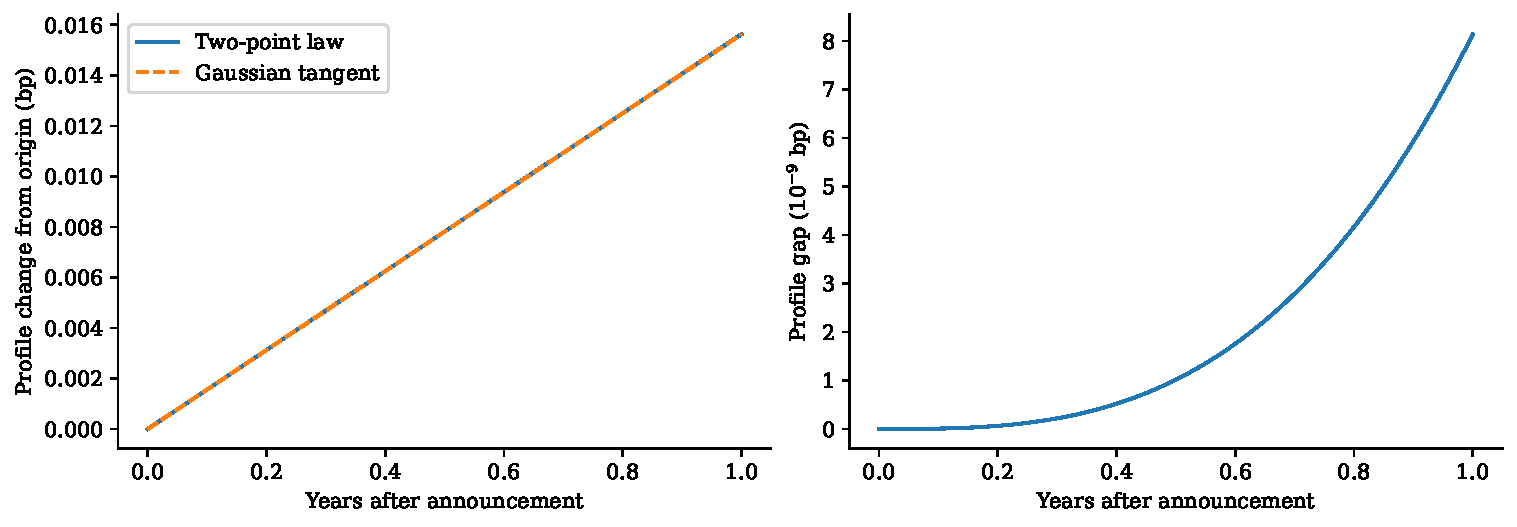
\includegraphics[width=\linewidth]{figures/jump_profiles.pdf}
\caption{Admissible profiles for a symmetric two-point level shock and its Gaussian tangent. The left panel subtracts the common value at zero; the right panel resolves the difference hidden at the scale of the left panel.}\label{fig:jumps}
\end{figure}

\subsection{A small exact recurrent model}
Take $a_i=1-\theta^i$, $0<\theta<1$, and $\lambda(x)=\eta e^{-\kappa x}$. A convenient representation is
\[
u=(1,-1),\quad M=\diag(1,\theta),\quad v=(1,1)^\top,
\qquad c=\eta,\quad A=-\kappa,\quad b=1.
\]
Here $d_*=2$, so \eqref{eq:state} has two $\Xi$ coordinates, three symmetric $\Pi$ coordinates, and two $\Theta$ coordinates. Under constant scale only the two $\Xi$ coordinates are random. Increasing the number of meetings changes $\mathcal D$ and the restart times, but adds no coordinates.

The loadings satisfy $a_{i+2}=(1+\theta)a_{i+1}-\theta a_i$. Their Hankel matrices have rank at most two, and rank exactly two once both independent components are visible. Figure~\ref{fig:hankel} contrasts this example at $\theta=0.7$ with cumulative harmonic loadings. A rapidly falling numerical singular-value spectrum is not a proof of exact finite rank; the distinction between approximation and exact realization is precisely the distinction needed here.
\begin{figure}[htbp]
\centering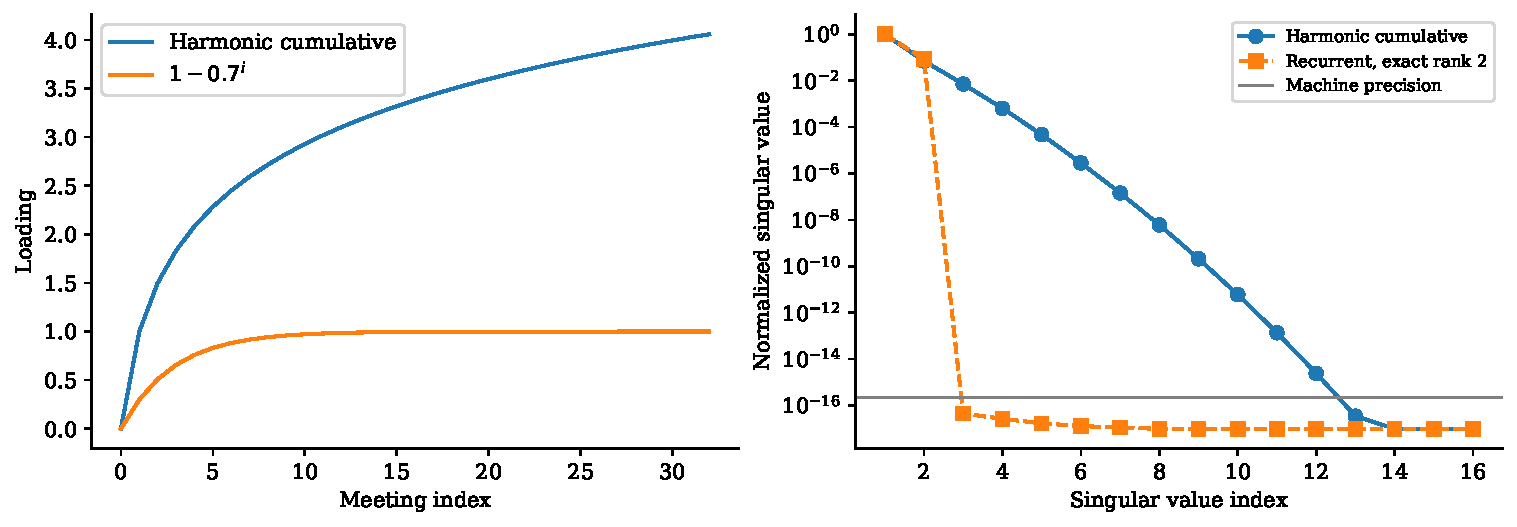
\includegraphics[width=\linewidth]{figures/hankel.pdf}
\caption{Loadings and singular values of their $16\times16$ Hankel sections. The recurrent example has exact rank two. The harmonic sequence is not recurrent, although its finite sections have rapidly decaying singular values. Values close to machine precision should not be interpreted as exact ranks.}\label{fig:hankel}
\end{figure}

\subsection{Compressing harmonic loadings on a calendar}
For integer $i\ge0$,
\begin{equation}
a_i=\sum_{j=1}^i\frac1j=\int_0^1\frac{1-x^i}{1-x}\dd x.
\label{eq:harmonicint}
\end{equation}
Choose $n_q$ Gauss--Legendre nodes $x_j\in(0,1)$ and weights $w_j>0$ on $[0,1]$. The approximation
\begin{equation}
\widetilde a_i=\sum_{j=1}^{n_q}\frac{w_j}{1-x_j}(1-x_j^i)\label{eq:quadraturerecurrence}
\end{equation}
is a sum of a constant and $n_q$ geometric sequences. It therefore has recurrence order at most $n_q+1$, and is bounded as $i\to\infty$ for each fixed $n_q$. The polynomial identity in \eqref{eq:harmonicint} also explains why the first few entries are particularly accurate. The example chooses the number of quadrature nodes and measures the resulting error on the calendar of interest.

Use a four-year horizon with 32 equally spaced meetings strictly inside it, zero initial curve, and $\lambda(x)=0.0025e^{-0.35x}$. Compare forward and bond prices at $t=2$, $T=4$. The maximum loading error is computed over indices $0$ through $32$; Theorem~\ref{thm:approximation} converts it into forward and price bounds. Here we use the sharper pointwise bounds at the chosen observation time and maturity. Table~\ref{tab:approx} compares those bounds with the pointwise Gaussian errors. Forward errors are in basis points of rate; bond errors are $10^4$ times absolute price errors for unit notional.

\begin{table}[htbp]\centering\small
\begin{tabular}{rrrrrr}
\toprule
Order & $\varepsilon$ & Forward RMSE & Bound & Bond RMSE & Bound\\
\midrule
\csname @@input\endcsname examples/results.tex 
\bottomrule
\end{tabular}
\caption{Recurrent approximation on the specified 32-meeting calendar. Orders are upper bounds. Both the bounds and the measured errors are evaluated at $(t,T)=(2,4)$.}\label{tab:approx}
\end{table}

The maturity integrals are evaluated analytically on each meeting interval. Remaining deterministic time integrals use Gauss--Legendre quadrature split at meetings; doubling from 12 to 24 nodes per interval checks numerical convergence. The errors use Gaussian moment formulas, not Monte Carlo estimates. In particular, write the Gaussian log prices as $\ell_P=\log P$ and $\widetilde\ell_P=\log\widetilde P$. Set $\delta_P=\ell_P-\widetilde\ell_P$, $v_P=\Var\delta_P$, and $b_P=\E\delta_P+v_P/2+2\Cov(\delta_P,\widetilde\ell_P)$. Then
\[
\E(P-\widetilde P)^2
 =e^{2\E\widetilde\ell_P+2\Var\widetilde\ell_P}
 \{(e^{b_P}-1)^2+e^{2b_P}(e^{v_P}-1)\}.
\]
Using \texttt{expm1} in this expression avoids cancellation when the approximation is accurate.

\begin{figure}[htbp]
\centering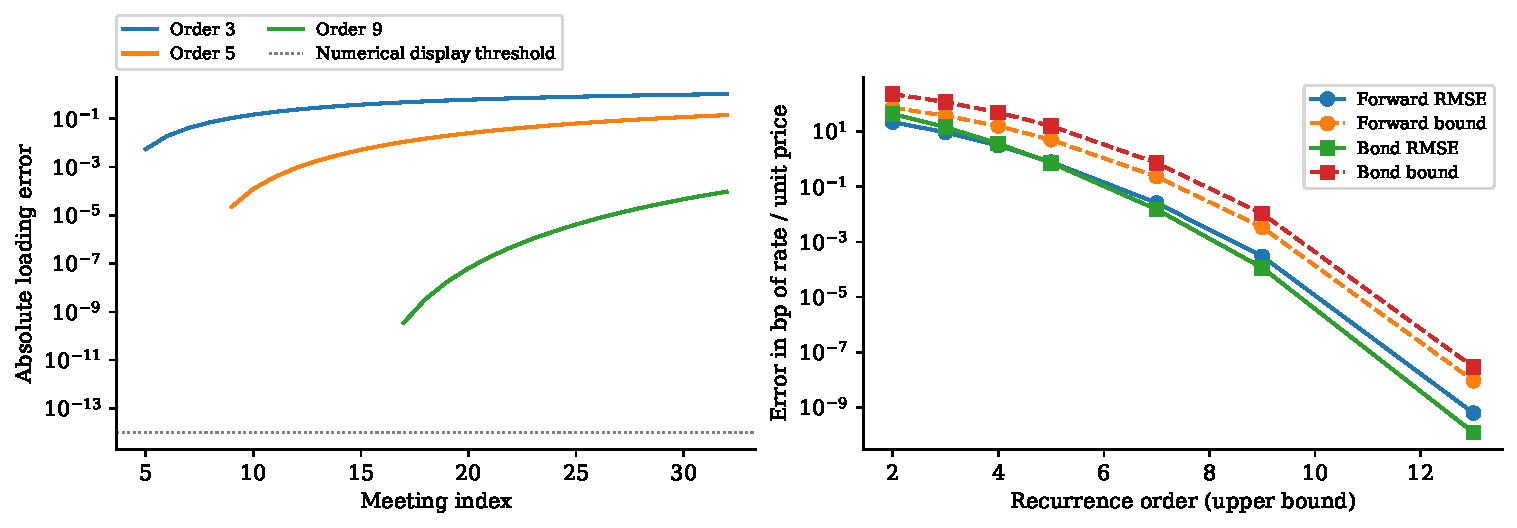
\includegraphics[width=\linewidth]{figures/approximation.pdf}
\caption{Loading approximation and resulting Gaussian forward and bond errors. Dashed curves are the bounds of Theorem~\ref{thm:approximation}; solid curves are computed pointwise errors. Loading errors below $10^{-14}$ are omitted and the numerical display threshold is marked. The comparison uses a fixed finite index range.}\label{fig:approximation}
\end{figure}

\subsection{A forbidden correlation made visible}
Consider a front-end volatility with one step of size $\Delta s$ at $\tau$, and an exponential block volatility $\eta_B e^{-\kappa(T-u)}$, with driver correlation $\rho$. Their aggregate step covariance is $\rho \eta_B\Delta s$, which violates \eqref{eq:steporth} when nonzero. For an observation time $t<\tau$, the difference of the adjacent analytic cross-term extensions, integrated from time zero to $t$, is
\begin{equation}
\mathcal R_\rho(T)=c_\rho e^{-\kappa T}(T-\tau-1/\kappa)+\rho \eta_B\Delta s\,t/\kappa,
\qquad c_\rho=\rho \eta_B\Delta s\frac{e^{\kappa t}-1}{\kappa}.\label{eq:numericcross}
\end{equation}
It is not affine when the covariance is nonzero. Figure~\ref{fig:splice} uses $t=0.5$, $\tau=1$, $\kappa=0.6$, $\eta_B=0.008$, $\Delta s=0.007$, and $\rho=0.6$. Subtracting the affine tangent at the meeting leaves a curved remainder. The remainder displays the shape that a piecewise-linear drift cannot absorb. Thus the figure diagnoses why this proposed correlation is incompatible with the chosen curve family.
\begin{figure}[htbp]
\centering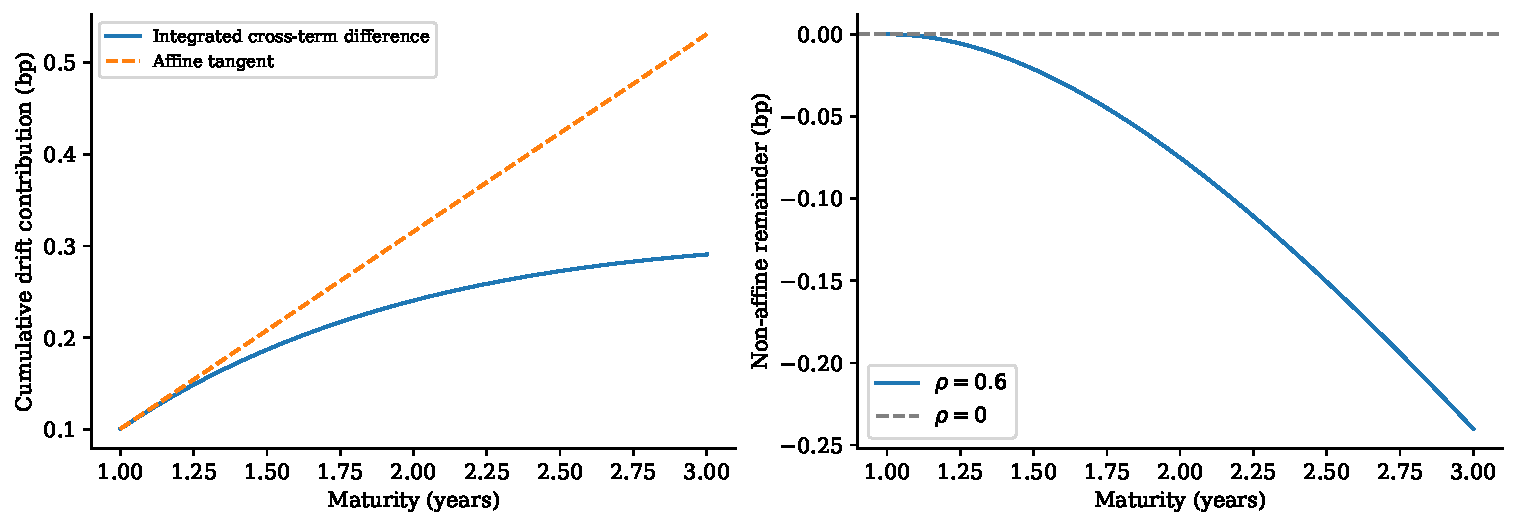
\includegraphics[width=\linewidth]{figures/splice_correlation.pdf}
\caption{A correlation that the stipulated splice cannot accommodate. The residual curvature vanishes when $\rho=0$. A smooth global block and an intervalwise affine front end cannot absorb different non-affine analytic expressions on adjacent intervals.}\label{fig:splice}
\end{figure}

For an eventual fitting procedure, the structural order is clear: choose an admissible block and recurrence class, enforce their covariance restrictions, compute each model's HJM drift, and only then fit loading and scale parameters. The resulting fit would then measure approximation within a class whose dynamics satisfy the structural restrictions.

\section{Conclusion}
A scheduled-date curve model has to answer three structural questions: what happens when information arrives, how past shocks are stored, and how meeting effects interact with the rest of the curve. The bond-price drift and announcement conditions link each answer to the chosen maturity shapes.

For announcements, a prescribed correction across maturities determines a conditional exponential moment of the level change. A linear correction leads to a Gaussian law, with the appropriate change of measure on later intervals. For continuous dynamics, a finite recurrence of the meeting loadings permits past shocks to be stored in a state whose size does not grow with the calendar. Without such a recurrence, an exact state of fixed size is impossible in the constant-scale setting studied here. On a finite calendar, a recurrent approximation can nevertheless be accurate, and the loading error supplies explicit bounds for forward rates and bond prices.

For a meeting-related curve added to a smooth component, covariance matters through the drift. The change in volatility at each meeting must be uncorrelated with the nonconstant smooth coordinates, and the remaining smooth drift restriction must use the combined level noise. These conditions give a direct way to check a proposed combination and to construct its front-end drifts. The Svensson calculation makes the permitted extra level correlation explicit. Allowing positive decay parameters to move does not remove the standalone block restrictions in an uncorrelated splice: its entire residual must still vanish.

The three-exponent construction supplies a positive stochastic-volatility example: variance is recovered from three forward rates, and discounted bonds are true martingales. It uses fixed exponents, one maturity breakpoint, and no diffusion after that date. This complements the restrictions without establishing a general classification of curve-dependent variance laws.

The examples show why exact and numerical questions should be examined together. A discrete hike/no-hike announcement is exactly excluded by the piecewise-affine jump family, but its required correction can be almost identical to the Gaussian one at realistic rate scales. A loading sequence can fail every exact finite recurrence yet admit an accurate low-order approximation on a given calendar. These distinctions make the structural results useful both for selecting a model family and for deciding how much complexity an implementation needs.

Three questions remain. The smallest autonomous state dimension under our calendar convention is not determined. The finite-calendar announcement construction does not establish a uniform-state realization theory with scheduled jumps. Finally, the numerical examples are synthetic: market calibration and assessment against observed prices remain to be carried out.

\appendix
\section{Supporting proofs}\label{app:proofs}
\subsection{Tilted Gaussian marginals without joint Gaussianity}
Take two maturity intervals, lengths $\ell_1,\ell_2>0$, and deterministic $y_1,y_2>0$. Under an auxiliary measure $Q_*$ let $X_1\sim N(-\ell_1y_1,y_1)$ and let $Z\sim N(0,y_2)$ be independent. Define
\[
X_2=\operatorname{sign}(X_1+\ell_1y_1)|Z|,
\qquad \frac{\dd Q}{\dd Q_*}=\exp(\ell_1X_1+\tfrac12\ell_1^2y_1).
\]
The density has expectation one. Under $Q$, $X_1\sim N(0,y_1)$. Tilting $Q$ by $\exp(-\ell_1X_1-\tfrac12\ell_1^2y_1)$ recovers $Q_*$, under which the sign in the definition of $X_2$ is an independent fair sign relative to $|Z|$. Consequently $X_2\sim N(0,y_2)$ under the second tilted measure, as required by Theorem~\ref{thm:tilts}.

Under $Q$, however, $Q(X_2>0)=Q(X_1>-\ell_1y_1)>1/2$. The magnitude retains the half-normal distribution and is independent of that sign. Its density is different constant multiples of the same centered Gaussian density on the two half-lines, with a discontinuity at zero. It is not Gaussian, and the pair cannot be jointly Gaussian. This supplies a nontrivial example rather than merely observing that marginal normality need not imply joint normality.

\subsection{The observability step in the splice proof}
The following elementary argument is applied with $(C,A)=(\mathcal C,\mathcal A)$ in the splice proof.
Let $A$ be invertible, $(C,A)$ observable, and suppose
\[
C e^{Ax}\{(x-a)I+A^{-1}\}v=0
\]
on an open interval. By real analyticity the identity holds for all real $x$. Put $g(x)=C e^{Ax}A^{-1}v$. The identity says $(x-a)g'(x)+g(x)=0$, so the derivative of $(x-a)g(x)$ vanishes. Its value at $x=a$ is zero. Thus $g(x)=0$ away from $a$, and by continuity also at $a$. Derivatives at zero give $CA^kA^{-1}v=0$ for all $k\ge0$. Observability implies $A^{-1}v=0$ and hence $v=0$.

This proof does not require diagonalizability. Diagonalizability is needed only for the stronger polynomial--exponential orthogonality in Corollary~\ref{cor:diagonal}, where positive powers multiplying an eigen-exponential cannot already be supplied by the drift basis.

\subsection{The three-exponent stochastic-volatility construction}\label{app:varianceexample}
\begin{proof}[Proof of Proposition~\ref{prop:varianceexample}]
First solve the scalar equation for $Z_2$ before stopping. Its drift and diffusion are
\[
b(z)=\frac{\tanh z}{2\kappa},\qquad a(z)=\sqrt{2+\tanh z}.
\]
Both are bounded and globally Lipschitz, since
$|b'(z)|\le1/(2\kappa)$ and $|a'(z)|\le1/2$.
Strong existence and pathwise uniqueness give a solution adapted to the natural filtration of $W^2$. Stop it at $\tau$ and define $Z_1,Z_4$ by their explicit formulas. This also proves uniqueness of the full stopped system in the joint Brownian filtration. The bound $1<v<3$ gives all required finite-horizon integrability.

For $t<\tau\le T$, put $y=T-\tau$. The volatility integrals are
\[
\int_t^T\sigma_1(t,u)\dd u=\frac{1-e^{-\kappa y}}{\kappa},\qquad
\int_t^T\sigma_2(t,u)\dd u=\sqrt{v_t}\frac{1-e^{-2\kappa y}}{2\kappa}.
\]
Their products with the respective volatilities give the drift displayed after the proposition. At fixed $T$, the drift of \eqref{eq:threeexpcurve} is
\[
\frac{e^{-\kappa y}}{\kappa}
 +\frac{v_t-2}{2\kappa}e^{-2\kappa y}
 -\frac{v_t}{2\kappa}e^{-4\kappa y},
\]
which agrees. For $T<\tau$ or $t\ge\tau$ the fixed-maturity coefficients have zero dynamics. There is no fixed-maturity curve jump at $\tau$, so the announcement condition is automatic.

For $k\in\{1,2,4\}$ and $T\ge\tau$ define
$A_k(T)=(1-e^{-k\kappa(T-\tau)})/(k\kappa)$.
Before $\tau$, $B_t=1$ and $P(t,T)=\exp(-\sum_k Z_k(t)A_k(T))$.
The integrated drift identity reads
\[
\frac{A_1}{\kappa}+\frac{v-2}{2\kappa}A_2-\frac{v}{2\kappa}A_4
       =\frac12(A_1^2+vA_2^2).
\]
It\^o's formula therefore gives
\[
\frac{\dd(P(t,T)/B_t)}{P(t,T)/B_t}
 =-\ind_{\{t<\tau\}}\{A_1(T)\dd W^1_t+\sqrt{v_t}A_2(T)\dd W^2_t\}.
\]
After $\tau$, direct integration of the frozen curve gives
\[
\log P(t,T)=-\sum_{k\in\{1,2,4\}}Z_k(\tau)
  \frac{e^{-k\kappa(t-\tau)}-e^{-k\kappa(T-\tau)}}{k\kappa}.
\]
Its time derivative is $r_t$, so the discounted bond is constant there, with the same value at $\tau$ as the preceding formula. The driving martingale has quadratic variation bounded by
$\tau(\kappa^{-2}+3/(4\kappa^2))=7\tau/(4\kappa^2)$.
The exponential-martingale criterion consequently makes the discounted bond a true martingale. For $T<\tau$ it is identically one.

The quadratic variation of $Z_2$ is $v_t\dd t$ before $\tau$; It\^o's formula for $2+\tanh Z_2$ gives the stated strictly positive density of $[v]$. The three curve evaluations have coefficient matrix
\[
\begin{pmatrix}
1&1&1\\[2pt]
1/2&1/4&1/16\\[2pt]
1/4&1/16&1/256
\end{pmatrix},\qquad \det=-21/1024.
\]
They therefore recover $Z_1,Z_2,Z_4$ and $v$.

Finally $r_{\tau-}=0$, and summing the three state equations cancels their drift, giving \eqref{eq:varianceexamplejump}. The integral with respect to $W^2$ is measurable with respect to that Brownian path. Conditional on this path, the jump is a translate of the independent $N(0,\tau)$ variable $W^1_\tau$. Its probability of being zero is therefore zero. This proves the last assertion without assuming that the second integral is Gaussian.
\end{proof}

\subsection{The Svensson covariance calculation}\label{app:svensson}
\begin{proof}[Proof of Corollary~\ref{cor:svensson}]
Expand \eqref{eq:residual} using the four basis functions
$1,e^{-\beta_1x},xe^{-\beta_1x},xe^{-\beta_2x}$.
Distinct exponential factors multiplied by polynomials are linearly independent. Every coefficient at a nonzero exponent must therefore vanish if $R$ is affine.

First consider the fourth covariance row. If $2\beta_2\ne\beta_1$, the coefficient of $x^2e^{-2\beta_2x}$ is $\mathsf Q_{44}/\beta_2$, hence $\mathsf Q_{44}=0$. If instead $2\beta_2=\beta_1$, the coefficient of $x^2e^{-2\beta_1x}$ first gives $\mathsf Q_{33}/\beta_1=0$. Positive semidefiniteness makes the third row zero. The coefficient of $x^2e^{-\beta_1x}$ is then $\mathsf Q_{44}/\beta_2-\mathsf Q_{13}=\mathsf Q_{44}/\beta_2$, again forcing zero. In both cases the fourth row vanishes by positive semidefiniteness.

If $\beta_2\ne2\beta_1$, the constant coefficient at exponent $-\beta_2$ is now $-z_4$: the time-to-maturity derivative contributes it, but neither the drift basis nor the remaining covariance products can cancel it. Thus $z_4\ne0$ precludes affinity.

In the resonant case $\beta_2=2\beta_1=2\beta$, the coefficient of $x^2e^{-2\beta x}$ is $\mathsf Q_{33}/\beta-\mathsf Q_{14}$. The fourth row is already zero, so the third row also vanishes. The constant and linear terms at exponent $-2\beta$ then give
\[
-z_4+\mathsf Q_{22}/\beta=0,\qquad \mu_4+2\beta z_4=0.
\]
The remaining coefficients at exponent $-\beta$ give
\[
\mu_2-z_3+\beta z_2+\mathsf Q_{12}/\beta-\mathsf Q_{22}/\beta=0,
\qquad \mu_3+\beta z_3-\mathsf Q_{12}=0.
\]
These are exactly \eqref{eq:svenssoncov}. The only residual is
$\mu_1-\mathsf Q_{12}/\beta-\mathsf Q_{11}x$.
The surviving two-by-two covariance block is positive semidefinite exactly under the inequalities in the corollary. Conversely, substituting all these conditions cancels every nonzero-exponent term. If $R=0$ is required, its slope gives $\mathsf Q_{11}=0$, positive semidefiniteness gives $\mathsf Q_{12}=0$, and its constant gives $\mu_1=0$.
\end{proof}

\clearpage
\section{Notation}
Symbols used only inside a proof are defined there. The principal model quantities are collected below. Polynomial powers use integer indices $j,k$; $\mu$ is reserved for drift coefficients and $\nu$ for block noise rows.

{\small
\begin{longtable}{p{.31\linewidth}p{.60\linewidth}}
\toprule
Symbol & Meaning\\
\midrule
\endfirsthead
\toprule
Symbol & Meaning (continued)\\
\midrule
\endhead
\bottomrule
\endfoot
$t,T,x=T-t$ & Observation time, maturity, and time to maturity.\\
$H,T_n,I_m,j(t)$ & Horizon, meeting dates, maturity intervals, and current interval index.\\
$Q,\E,W$ & Pricing measure, its expectation, and Brownian driver.\\
$f,P,r,B$ & Forward rate, bond price, short rate, and bank account.\\
$\alpha,\sigma,\xi_n$ & Forward drift, Brownian sensitivity, and announcement change.\\
$h,h_0,\mathcal H$ & Jump correction, its affine intercept, and its maturity integral.\\
$\mathcal L_X$ & Conditional log-Laplace transform of the level change.\\
$\ell_k,X_k,y_k$ & Interval length, announcement level, and announcement slope.\\
$\bar x_k,\Sigma$ & Jointly Gaussian announcement mean and covariance.\\
$\mathcal U_k,\mathcal Z_k,Q_k$ & Earlier-interval jump integral, tilt density, and tilted measure.\\
$s_k,\mu_k^L,\mu_k^C$ & Step volatility and required level and slope drifts.\\
$\mathcal V_k^S$ & Volatility integrated up to the start of interval $I_k$, or zero on the current interval.\\
$a_i,\lambda(x)$ & Meeting-loading sequence and smooth maturity function.\\
$\mathcal D(t),i(t,T)$ & Remaining meeting distances and number of intervening meetings.\\
$A,b,c;d_\lambda$ & Matrix-exponential representation of $\lambda$ and its dimension.\\
$M,u,v;p$ & Matrix representation of the recurrence and its dimension.\\
$\Xi,\Pi,\Theta;d_*=p d_\lambda$ & Realization states and combined vector size.\\
$k,\mathcal I,\mathcal V_a$ & Curve-evaluation row, its maturity integral, and integrated unscaled volatility.\\
$\mathsf H_{R,n},q$ & Finite loading Hankel section and total state dimension.\\
$\varepsilon,\bar a,\Lambda$ & Maximum loading error, loading magnitude, and shape magnitude.\\
$C_H,B_{t,T},E_{t,T}$ & Uniform log-price bound, pointwise log-price bound, and price-moment exponent.\\
$L_m,C_m,V_m,G_m$ & Front-end level, slope, noise row, and maturity-step change of that row.\\
$F,Z,\mathcal A,\mathcal C;d_B$ & Smooth block, coefficient process, exponential representation, and exponential block dimension.\\
$\mu_k,\nu^k,\mathsf Q$ & Block coordinate drift, noise row, and covariance matrix.\\
$\varphi_k,\Phi_k$ & Block coordinate function and its maturity integral.\\
$\Sigma^S,\Sigma^B,\chi_m$ & Integrated front-end and block volatilities, and interval constant in $\Sigma^S=TV_m+\chi_m$.\\
$\mathcal K_m,\bar\omega_k$ & Covariance cross term on $I_m$ and covariance of block coordinate $k$ with current front-end noise.\\
$R,R_\sharp,\mathcal X$ & Block residual, adjusted residual, and common non-level cross term.\\
$\mu_m^S$ & Required front-end drift on interval $I_m$.\\
$\kappa,\theta,\rho,\pi,n_q$ & Exponential decay rate, geometric ratio, driver correlation, two-point probability, and quadrature-node count.\\
$\ell_P,\delta_P,v_P,b_P$ & Log price, log-price difference, its variance, and exponent in the numerical Gaussian moment formula.\\
$\tau,Z_1,Z_2,Z_4,v_t$ & Single scheduled date, three exponential coefficients, and variance $2+\tanh Z_2(t)$ in Section~\ref{sec:varianceexample}.\\
$\beta_i,p_i,p_{[i]},R_{\rm var}$ & Decay parameters, their coefficient polynomials, sums for coinciding decays, and the nonlinear block residual in Section~\ref{sec:varyingexponents}.\\
$\mathcal R_\rho,c_\rho$ & Integrated cross-term difference and its exponential coefficient in the correlation example.\\
\end{longtable}
}

\bibliographystyle{plainnat}
\bibliography{refs}
\end{document}
